% !TEX program = xelatex
% =============================================================================
%  华数杯数学建模竞赛 LaTeX 模板
%  对应 Typst 模板 zh/huashubei/main.typ 的全部功能。
%
%  字体依赖（正文宋体 / 标题黑体 / 强调楷体）：
%    - 规范字体：SimSun（宋体）、SimHei（黑体）、KaiTi（楷体）。
%    - 本模板使用 ctex 的 fontset=windows，在 Windows 上使用规范字体
%      SimSun / SimHei / KaiTi，确保开箱即用。
%    - 若系统已安装 SimSun/SimHei/KaiTi（如 Windows 或手动安装），当前设置可直接使用。
%    - 西文正文：Times New Roman；代码等宽：Consolas。
%  编译方式：xelatex main.tex
% =============================================================================
\documentclass[fontset=windows, 12pt, a4paper]{ctexart}

% ---------- 页面：A4，上下左右 2.5cm ----------
\usepackage[a4paper, top=2.5cm, bottom=2.5cm, left=2.5cm, right=2.5cm]{geometry}

% ---------- 数学 ----------
\usepackage{amsmath}
\usepackage{url}
\usepackage{ragged2e}

% ---------- 表格跨行 & 基础表格工具 ----------
\usepackage{multirow}
\usepackage{booktabs}
\usepackage{array}
\usepackage{graphicx}
\usepackage{float}
\usepackage{tabularx}   % tabularx 和 X 列
% 压缩图表和正文之间空白
\setlength{\intextsep}{5pt plus 1pt minus 1pt}
% 标题 ↔ 表格/图片距离
\setlength{\abovecaptionskip}{3pt}
\setlength{\belowcaptionskip}{3pt}
\graphicspath{{figures/}}
% ---------- 字体（fontspec + ctex，xelatex 编译） ----------
\IfFontExistsTF{Times New Roman}{\setmainfont{Times New Roman}}{}
\IfFontExistsTF{Consolas}{\setmonofont{Consolas}}{}

% ---------- 正文：12pt，首行缩进 2em，两端对齐，行距 0.92em ----------
% 0.92em 行距 => 行高 = 1.92 * 字号，\linespread 因子 ≈ 1.6
\linespread{1.6}
\setlength{\parindent}{2em}

% ---------- 标题编号（\ctexset 配置） ----------
% 一级标题用中文数字“一、二、三、”，二级及以下用 1.1 / 1.1.1
\ctexset{
	section/number       = \chinese{section},
	subsection/number    = \arabic{section}.\arabic{subsection},
	subsubsection/number = \arabic{section}.\arabic{subsection}.\arabic{subsubsection},
}

% ---------- 标题格式（titlesec 配置） ----------
% 对应 Typst：一级 14pt 居中黑体加粗，二级 12pt 黑体加粗，三级 12pt 黑体加粗
\usepackage{titlesec}
\titleformat{\section}
{\centering\fontsize{14pt}{16.8pt}\heiti\bfseries}
{\chinese{section}、}{1em}{}
\titleformat{\subsection}
{\fontsize{12pt}{14.4pt}\heiti\bfseries}
{\arabic{section}.\arabic{subsection}}{1em}{}
\titleformat{\subsubsection}
{\fontsize{12pt}{14.4pt}\heiti\bfseries}
{\arabic{section}.\arabic{subsection}.\arabic{subsubsection}}{1em}{}
\titlespacing{\section}       {0pt}{1.0em}{-0.50em}
\titlespacing{\subsection}    {0pt}{1.18em}{-0.50em}
\titlespacing{\subsubsection} {0pt}{0.9em}{0.75em}

% ---------- 列表（enumitem）：对应 Typst enum 编号“1、 2、”，缩进 2em ----------
\usepackage{enumitem}
% ---------- 列表（enumerate） ----------
\usepackage{enumitem}
\setlist[enumerate]{
	label=\arabic*、,
	leftmargin=2.2em,     % 整个列表距离正文左边的位置
	labelsep=0.35em,      % 编号“1、”与正文之间的距离
	itemsep=0em,       % 不同条目之间的距离
	topsep=0.25em,        % 列表与上、下正文之间的距离
	parsep=0pt,           % 同一条目内部不同段落的额外距离
	partopsep=0pt
}

% ---------- 代码与颜色 ----------
\usepackage{xcolor}
\usepackage{listings}
\lstset{
	basicstyle=\ttfamily\small,
	backgroundcolor=\color{black!3},
	frame=single,
	framesep=6pt,
	rulecolor=\color{black!30},
	framerule=0.8pt,
	breaklines=true,
	showstringspaces=false,
	columns=fullflexible,
	keepspaces=true,
}

% ---------- 页码：底部居中（华数杯从首页开始编号） ----------
\pagestyle{plain}

% ---------- 自定义命令（对应 Typst 函数） ----------
% \referencescn：参考文献节，标题“参考文献”（不带编号）
\newcommand{\referencescn}{%
	\begin{thebibliography}{99}
	\RaggedRight
	
	% 参考文献间距压缩
	\setlength{\itemsep}{0pt}
	\setlength{\parskip}{0pt}
	\setlength{\parsep}{0pt}
	
	% 单独设置参考文献行距
	\linespread{1.5}\selectfont
	
	\setlength{\emergencystretch}{2em}
	
	\bibitem{ref1}
	王继业，周碧玉，张法，等，数据中心能耗模型及能效算法综述，
	计算机研究与发展，56(8)：1587--1603，2019。	
	\bibitem{ref2}
	丁肇豪，曹雨洁，张素芳，等，能源互联网背景下数据中心与电力系统协同优化（一）：数据中心能耗模型，
	中国电机工程学报，42(9)：3161--3176，2022。	
	\bibitem{ref3}
	吕佳炜，张沈习，程浩忠，等，集成数据中心的综合能源系统能量流--数据流协同规划综述及展望，
	中国电机工程学报，41(16)：5500--5521，2021。
	
	\bibitem{ref4}
	Wickramasuriya S L, Athanasopoulos G, Hyndman R J,
	Optimal Forecast Reconciliation for Hierarchical and Grouped Time Series Through Trace Minimization,
	Journal of the American Statistical Association, 114(526): 804--819, 2019.
	
	\bibitem{ref5}
	Radovanovic A, Koningstein R, Schneider I, et al.,
	Carbon-Aware Computing for Datacenters,
	IEEE Transactions on Power Systems, 38(2): 1270--1280, 2023.
	
	\bibitem{ref6}
	Lindberg J, Lesieutre B C, Roald L A,
	Using Geographic Load Shifting to Reduce Carbon Emissions,
	Electric Power Systems Research, 212: 108586, 2022.
	
	\bibitem{ref7}
	Guo X, Che Y, Zheng Z, et al.,
	Multi-timescale Optimization Scheduling of Interconnected Data Centers Based on Model Predictive Control,
	Frontiers in Energy, 18(1): 28--41, 2024.
	
	\bibitem{ref8}
	Liu W, Yan Y, Sun Y, et al.,
	Online Job Scheduling Scheme for Low-carbon Data Center Operation: An Information and Energy Nexus Perspective,
	Applied Energy, 338: 120918, 2023.
	
	\bibitem{ref9}
	向梓旸，黄淳驿，李康平，等，考虑负载时空转移特性的数据中心集群算电协同优化调度，
	电力信息与通信技术，24(3)：33--46，2026。
	
	\bibitem{ref10}
	Wang K, Ye L, Yang S, et al.,
	A Hierarchical Dispatch Strategy of Hybrid Energy Storage System in Internet Data Center with Model Predictive Control,
	Applied Energy, 331: 120414, 2023.

	\bibitem{ref11}
	DeepSeek, DeepSeek-v4-flash-0731, 深度求索 (DeepSeek), 使用日期：2026-08-07--2026-08-10.
	
\end{thebibliography}
%
}
% \appendixcn：附录节，标题“附录 A  核心代码”
\newcommand{\appendixcn}{%
	\section*{附录 A\quad 核心代码}%
	\section*{附录}

\subsection*{A. 软件环境与复现说明}

本文采用Python 3.12.13完成计算，使用NumPy、pandas、Matplotlib、Seaborn、OpenPyXL、SciPy和HiGHS完成科学计算、数据处理、绘图和优化求解，使用\texttt{uv}管理运行环境。依赖约束和锁定信息见支撑材料中的\texttt{pyproject.toml}与\texttt{uv.lock}。

复核时先同步运行环境，再按问题一至问题四的顺序执行题目级入口。问题二至问题四的预处理依赖问题一生成的共享处理层，因此不将项目根目录的\texttt{main.py}作为无条件复现入口。运行命令如下：

\begin{lstlisting}[language={},basicstyle=\ttfamily\small]
uv sync
uv run python question\question_01\main.py
uv run python question\question_02\main.py
uv run python question\question_03\main.py
uv run python question\question_04\main.py
\end{lstlisting}

各题入口依次完成数据处理、模型求解、模型检验和结果绘图。支撑材料中同时保留了处理后的模型输入和已生成的结果表。若仅复核论文中的数值，可直接检查结果表及独立检验表；若要从原始附件重新计算，应在保持题目数据不变的前提下重新完成数据处理。

\subsection*{B. 源程序与支撑材料}

支撑材料包含本题全部计算机源程序、运行环境配置、处理后的模型输入、问题一至问题四的关键结果表、模型检验表、论文图形以及文件校验清单。结果表用于追溯正文中的具体数值，图形用于论文展示，独立检验表用于核对任务覆盖、资源容量、能源平衡、储能状态和时间边界等条件。

各问题的支撑结果分别包括：问题一的需求预测、基础算力调度和压力边界检验；问题二的多目标调度、基线对比、资源能源复算和敏感性检验；问题三的储能优化、区域指标、基准复核和约束检验；问题四的算力--储能--电力联合调度、情景比较、代表窗口检验和独立核验。

\subsection*{C. 结果使用边界}

正文中的数值以对应结果表为准，不从图片估读。通过硬约束检验只能说明当前方案在给定数据、参数和边界下具有可行性，不能单独推出全局最优或对所有场景普遍最优。对于采用数学启发式得到的结果，正文如实说明其求解方法、对照检验和剩余局限。

时间边界统一解释为：0--2399小时为主要运行期，2400--2405小时用于处理已到达任务的尾部执行，2406小时为终端结算时点，不作为普通任务运行小时。成本指标若包含售电收益，应按净结算值解释，不等同于实际用电量为负。

\subsection*{D. AI工具使用详情}

本参赛队在竞赛过程中使用了DeepSeek，主要用于语言润色、代码调试、图表制作与LaTeX排版辅助。AI未用于确定核心模型、公式、参数、原始数据和最终结论。

\subsubsection*{D.1 工具与使用日期}

\begin{table}[H]
    \centering
    \small
    \renewcommand{\arraystretch}{1.05}
    \setlength{\tabcolsep}{3pt}
    \begin{tabularx}{0.96\textwidth}{>{\centering\arraybackslash}p{0.18\textwidth}>{\centering\arraybackslash}p{0.20\textwidth}>{\centering\arraybackslash}X>{\centering\arraybackslash}p{0.22\textwidth}}
        \toprule
        AI工具 & 版本/型号 & 开发机构 & 使用日期 \\
        \midrule
        DeepSeek & DeepSeek-v4-flash-0731 & 深度求索（DeepSeek） & 2026年8月7日至8月10日 \\
        \bottomrule
    \end{tabularx}
\end{table}

本文使用的模型版本为DeepSeek‐v4‐flash‐0731。

\subsubsection*{D.2 使用环节与目的}

DeepSeek用于文字润色、程序调试、图表制作、终稿语言压缩、术语统一、正文引用、结果版本一致性检查和LaTeX排版复核。AI未用于生成或篡改原始数据，未改变既有联合任务搜索的目标函数、约束条件和参数设置；新增结果均由本地程序实际运行并独立复算。

\subsubsection*{D.3 关键交互记录}

\noindent\textbf{交互记录1（DeepSeek辅助润色，使用日期：2026年8月7日至10日）}

提示词要求：只检查由参赛队自行完成的论文文字，不增加新的模型、公式、数据或结论，并给出局部修改建议。AI主要指出长句、重复表述、术语不一致和图表衔接问题；参赛队人工筛选、核对并重新表述。

\noindent\textbf{交互记录2（代码调试与图表辅助，使用日期：2026年8月9日）}

提示词要求：仅检查已有程序的语法、索引、数据类型、文件读取和绘图参数，不修改原始数据、目标函数、约束条件、模型结构、参数设置和最终结论。AI提出变量检查、索引调整、数据类型转换和图表标签优化建议；参赛队仅采纳本地运行可复现且不改变模型含义的建议。

\noindent\textbf{交互记录3（DeepSeek终稿复核，使用日期：2026年8月10日）}

提示词要求：严格依据评审清单核对问题四的结果口径，消除顺序基准、联合方案、图表和正文之间的数据混用，并统一学术语体、文内引用和LaTeX排版。AI协助增加固定任务方案的统一能源定向复算与独立核验入口，修改绘图和论文源文件；所有新指标均由参赛队计算机本地运行生成，参赛队负责最终核对和提交。

\subsubsection*{D.4 采纳与人工修改}

AI建议均经参赛队核对后采纳。所有核心方法、公式、参数、结果和结论由参赛队确定；最终程序、数据、图表和结论由参赛队在本地运行并复核。DeepSeek完整记录见支撑材料中的相应使用报告。

程序中的AI辅助说明对应DeepSeek参与的代码检查与修改环节。AI辅助范围限于程序检查、结果复核、图表制作和论文排版，未改写既有联合任务搜索模型。

\subsection*{E. 源程序清单与附件位置}

本题实际使用的全部24个Python源程序不在论文附录中重复排印，统一收录于独立附件\texttt{CCM2601033附件.zip}的\texttt{源程序}目录。附件同时包含\texttt{pyproject.toml}、\texttt{uv.lock}、处理后的模型输入、关键结果表、模型检验表、论文图形及SHA-256校验清单，赛题提供的原始数据未重复收录。

源程序按问题一至问题四的相对目录组织，共24个\texttt{.py}文件；复核时按附录A所列命令依次运行。论文与附件分开提交，附件命名符合“选题+参赛编号+附件”的要求，压缩包大小控制在20 MB以内。
%
}
% \threelinetable{标题}{列定义}{表头}{表格内容}：三线表，标题在表格上方居中 10.5pt 黑体加粗
% 调用示例：\threelinetable{表 1 示例}{ccc}{A & B & C}{1 & 2 & 3 \\ 4 & 5 & 6}
\newcommand{\threelinetable}[4]{%
	\begin{center}
		{\fontsize{10.5pt}{12.6pt}\heiti\bfseries #1}\par
		\vspace{-0.5em}
		\begin{tabular}{#2}
			\toprule
			#3 \\
			\midrule
			#4 \\
			\bottomrule
		\end{tabular}
	\end{center}
}

\begin{document}
	
	% ---------- 官方模板顶部参赛信息表格 ----------
	% 直接压缩页面顶部边距，作用于整页顶部
%	\setlength{\topmargin}{-2.0cm}
%	\setlength{\headheight}{0pt}
%	\setlength{\headsep}{0pt}
	\begin{center}
		\renewcommand{\arraystretch}{1.25}
		\begin{tabularx}{\textwidth}{|>{\centering\arraybackslash}p{0.18\textwidth}|>{\centering\arraybackslash}X|>{\centering\arraybackslash}p{0.18\textwidth}|}
			\hline
			所属类别 
			& \multirow{2}{=}{\centering\fontsize{14pt}{16.8pt}\heiti\bfseries 2026年“华数杯”大学生数学建模竞赛} 
			& 参赛编号 \\
			\cline{1-1} \cline{3-3}
			本科组 
			& 
			& CM2601033 \\
			\hline
		\end{tabularx}
	\end{center}
	
	\vspace{-1.0em}
	
	% ---------- 标题与摘要页（页码从 1 开始） ----------
	\begin{center}
		{\fontsize{16pt}{19.2pt}\heiti\bfseries 多区域数据中心算储电协同的分层预测与多目标优化调度
		}
	\end{center}
	
	\vspace{-0.85em}
	
	\begin{center}
		{\fontsize{14pt}{16.8pt}\heiti\bfseries 摘\hspace{1em}要}
	\end{center}
	
	\vspace{-0.5em}
	
	针对六区域数据中心算电协同问题，构建“\textbf{分层预测与中性基线—碳感知调度—给定负荷下储能协同—算储电联合优化}”框架。
	
	对稀疏异质GPU需求采用三级\textbf{局部均值预测}，以\textbf{边际一致性}恢复18类交叉需求。取\textbf{72\,h历史窗口}，验证期、测试期WAPE为\textbf{0.7241、0.6519}，均优于24\,h同刻基线；
	538个任务经字典序调度实现\textbf{100\%本地执行}，累计等待\textbf{3\,h}。
	
	构建净运行成本、碳排放、网络时延和新能源未利用率\textbf{四指标模型}并\textbf{固定定标滚动求解}。较纯算力中性基准，
	净运行成本降低\textbf{507.34万元}、新能源利用率提高\textbf{0.2232个百分点}，
	但碳排放和平均网络时延分别增加\textbf{1.2752\,tCO$_2$、7.9468\,ms}。
	
	在题目给定的AI与非AI IT负荷下，依据\textbf{能量守恒、SOC递推和购售电边界}优化储能与购售电。
	与无储能反事实方案相比，净运行成本降低\textbf{3936.19万元}，
	碳排放由\textbf{8.8506\,tCO$_2$降至0}，
	六个区域峰值净购电之和由\textbf{31.5979\,MW降至0}。
	
	联合优化任务迁移、开工时刻、储能和购售电，建立包含成本、碳排放、网络时延、等待损失、新能源未利用率和峰值净购电的\textbf{六指标联合模型}，并基于\textbf{固定定标滚动求解}。为消除旧顺序能源解的退化影响，将顺序任务方案和联合任务方案均按相同能源口径复算。联合任务方案的净运行结算降低\textbf{65.67万元}，
	平均网络时延由\textbf{12.95\,ms降至9.96\,ms}，等待损失下降\textbf{0.004378}，新能源未利用率下降\textbf{0.0258个百分点}；
	相应地，碳排放和峰值净购电分别增加\textbf{41.08\,tCO$_2$、30.61\,MW}，体现服务质量、新能源消纳与能源侧指标之间的权衡。
	
	情景分析显示，强化碳约束减排\textbf{30.53\%--100\%}，固定区域均价使净运行成本增加\textbf{91.71万元}、峰值净购电增加\textbf{48.27\%}，非零出力时段完全平滑使碳排放降低\textbf{88.12\%}。
	
	\textbf{样本外检验与全时域独立复算}表明方案满足任务、资源、能量、SOC及购售电等硬约束。\textbf{滚动数学启发式得到严格满足硬约束且计算效率较高的可行方案，不宣称获得全局最优解}；
	联合决策量化呈现了成本、碳排放、服务质量、新能源消纳与削峰之间的权衡。
	
	\noindent\textbf{关键词：}算电协同；分层需求预测；碳感知调度；储能协同优化；多目标优化
	
	
	
	\newpage
	
	%\section{问题重述}
%
%\subsection{问题背景}
%
%数学建模是解决实际问题的重要工具。本文研究的问题涉及多维度数据分析与优化决策。
%
%\subsection{问题分析}
%
%\textbf{问题一：}对给定数据集进行分析和预测，要求模型具有泛化能力。
%
%\textbf{问题二：}考虑多因素影响，改进和优化模型，提高预测精度。
%
%\textbf{问题三：}结合实际约束条件，设计最优策略方案。
%
%\textbf{问题四：}结合实际约束条件，设计最优策略方案。
\section{问题重述}

\subsection{问题背景}

人工智能应用扩张使数据中心算力需求与能耗同步增长。数据中心能耗建模需同时考虑IT负荷、设施能效和电力交互\cite{ref1,ref2}，综合能源系统还需协调数据流与能量流\cite{ref3}。各区域的算力、电价、碳强度、新能源和网络时延不同，加之新能源波动及任务时限差异，形成跨区域、跨时段的算--储--电协同优化问题。


\subsection{问题分析}

\textbf{问题一：}预测第2376--2399小时各区域、各类任务的GPU需求；再以实际到达任务为对象，在时限、时延、GPU和功率约束下确定执行区域与开工时刻，形成基础算力基线。

\textbf{问题二：}在实际任务和能源参数下重新安排任务区域与开工时刻，建立兼顾运行成本、碳排放、网络时延和新能源利用率的碳感知调度模型。

\textbf{问题三：}固定题目给定的算力负荷，仅优化新能源分配、储能充放电和购售电，评价储能对成本、碳排放、峰值净购电及波动的影响。

\textbf{问题四：}联合优化任务调度、储能和购售电，在算力、能源与服务质量约束下比较联合方案、顺序基准及不同运行情景。


\subsection{整体技术路线}
如图\ref{fig:framework}，问题一形成纯算力基线，问题二引入电价、碳强度和新能源，问题三在固定负荷下考察储能，问题四联合开放任务与能源决策，构成“基础算力--算电协同--储能调节--算储电联合调度”的递进链路。


\begin{figure}[H]
	\centering
	\includegraphics[width=0.80\textwidth]{figures/华数杯流程图.pdf}
	\caption{多区域算--储--电协同优化整体技术路线}
	\label{fig:framework}
\end{figure}



	%\section{问题分析}
%
%\subsection{问题一的分析}
%
%问题一的关键在于特征工程和模型选择，数据中同时存在线性和非线性特征。
%
%\subsection{问题二的分析}
%
%问题二涉及多变量分析和模型融合技术，需要识别主要影响因素。
%
%\subsection{问题三的分析}
%
%问题三是约束优化问题，需要建立目标函数和约束条件。
%
%\subsection{问题四的分析}
%
%问题四

	\section{模型假设}

为统一各问建模口径，在题目给定条件基础上作如下假设：
\begin{enumerate}
	\item 任务一旦开始即连续执行，不可抢占、拆分或在运行过程中再次迁移。
	\item 任务开工时刻按整数小时确定；分钟级持续时间按照与各小时区间的实际重叠比例折算GPU及功率占用。
	\item AI IT功率按题目给定的统一功率映射计算，非AI IT负荷视为逐时已知且不可迁移。
	\item 跨区域任务仅考虑题目给定的网络时延，不额外计及网络带宽、迁移数据量及传输能耗。
	\item 各区域独立进行能源结算；储能同一时段不得同时充放电，并满足容量、充放电功率及终端SOC等约束。
\end{enumerate}

	\section{符号说明}

文中主要符号及含义如表\ref{tab:symbols}所示，
各问题中特有的参数和辅助变量在相应模型中另行说明。

\begin{table}[H]
	\centering
	\caption{主要符号说明}
	\label{tab:symbols}
	
	% 压缩表格字体和行距
	\small
	\renewcommand{\arraystretch}{0.85}
	
	\begin{tabularx}{0.96\textwidth}{
			>{\centering\arraybackslash}p{0.20\textwidth}
			>{\raggedright\arraybackslash}X
			>{\centering\arraybackslash}p{0.15\textwidth}}
		\toprule
		\textbf{符号} & \multicolumn{1}{c}{\textbf{含义}} & \textbf{单位} \\
		\midrule
		
		$i,r,t,s$
		& 任务、区域、时段及候选开工时刻索引
		& -- \\
		
		$a_i,e_i,o_i,d_i$
		& 到达、最早开工、最晚完成时刻及持续时间
		& h \\
		
		$g_i$
		& 任务$i$的GPU需求量
		& GPU \\
		
		$p_i$
		& 任务$i$的AI IT功率
		& MW \\
		
		$l_{ir},\,l_i^{\max}$
		& 执行时延及最大允许时延
		& ms \\
		
		$x_{irs}$
		& 任务$i$是否在区域$r$、时刻$s$开工
		& $\{0,1\}$ \\
		
		$\rho_{ist}$
		& 任务$i$在时段$t$内的运行占比
		& -- \\
		
		$P^{AI}_{rt},\,P^{NonAI}_{rt}$
		& AI IT负荷与非AI IT负荷
		& MW \\
		
		$F_{rt}$
		& 区域$r$的设施侧总负荷
		& MW \\
		
		$G^{ava}_{rt}$
		& 区域$r$的可用GPU容量
		& GPU \\
		
		$PUE_r$
		& 区域$r$的PUE
		& -- \\
		
		$P^{RE}_{rt}$
		& 区域$r$的可用新能源功率
		& MW \\
		
		$\pi_{rt},\,\sigma_{rt}$
		& 购电价格与售电价格
		& 元/MWh \\
		
		$\kappa_{rt}$
		& 电网碳强度
		& tCO$_2$/MWh \\
		
		$B_{rt},\,X_{rt},\,R_{rt}$
		& 电网购电、新能源外送及弃用功率
		& MW \\
		
		$S_{rt}$
		& 时段$t$开始时的储能电量
		& MWh \\
		
		\bottomrule
	\end{tabularx}
\end{table}


	%\section{问题一的模型建立与求解}
%
%\subsection{数据预处理}
%
%采用 Z-score 标准化处理：$x' = \frac{x - \mu}{\sigma}$。
%
%\subsection{模型建立}
%
%问题一包含GPU需求短期预测与基础算力调度两个相互独立的任务。
%预测部分利用第0--2375小时历史工作负载预测第2376--2399小时GPU需求；
%调度部分则直接使用第2376--2399小时实际到达任务，
%预测结果仅用于预测精度评价，不参与任务调度。
%
%首先按照“区域--任务类型--小时”统计GPU到达需求。
%设区域$r$、任务类型$k$在时刻$t$的新到达GPU需求为$D_{rkt}$，
%则有
%\begin{equation}
%	D_{rkt}
%	=
%	\sum_{\substack{i:\,ArrivalHour_i=t\\
%			SourceRegion_i=r,\;TaskType_i=k}}
%	GPU\_Demand_i .
%\end{equation}
%
%由此得到$6\times3=18$条底层需求序列。
%考虑到细粒度序列存在较多零值和随机尖峰，
%进一步构造区域需求$D_{rt}=\sum_kD_{rkt}$、
%任务类型需求$D_{kt}=\sum_rD_{rkt}$以及系统总需求
%$D_t=\sum_rD_{rt}$。
%其中18条底层序列用于刻画区域与任务类型异质性，
%而稳定性较高的区域层、任务类型层和系统层序列用于短期预测。
%
%对于任一聚合需求序列$y_t$，
%利用预测时点之前最近$H$小时的局部平均需求水平预测未来24小时，
%即
%\begin{equation}
%	\hat{y}_{T+h}(H)
%	=
%	\frac{1}{H}
%	\sum_{\tau=T-H+1}^{T}y_{\tau},
%	\qquad h=1,2,\ldots,24 .
%\end{equation}
%
%式(2)中，$T$为预测起点前最后一个已知时刻，
%$H$为历史窗口长度。
%在$H\in\{24,72,168,336\}$中，
%利用第2352--2375小时验证集选择预测窗口，
%模型确定后再使用第0--2375小时历史信息重新估计局部需求水平，
%对第2376--2399小时进行最终预测。
%该过程严格保持时间前向性，测试期真实数据不参与模型选择。
%
%由于区域需求、任务类型需求和系统需求分别预测后可能出现总量不一致，
%首先以系统总需求预测作为逐时总量锚点，
%对区域预测和任务类型预测进行比例调整，
%使二者的逐时总和均与系统预测一致。
%随后利用历史区域--任务类型需求结构$q_{rk}$恢复18类交叉需求。
%设恢复后的需求为$z_{rkt}$，则其满足
%\begin{equation}
%	\begin{aligned}
%		\min_{z_{rkt}\geq 0}\quad
%		&\sum_r\sum_k
%		z_{rkt}\ln\frac{z_{rkt}}{q_{rk}},\\
%		\mathrm{s.t.}\quad
%		&\sum_k z_{rkt}=\tilde{D}_{rt},\\
%		&\sum_r z_{rkt}=\tilde{D}_{kt}.
%	\end{aligned}
%\end{equation}
%
%其中，$\tilde{D}_{rt}$和$\tilde{D}_{kt}$分别表示一致性调整后的区域需求和任务类型需求。
%式(3)在保持两个边际预测结果不变的条件下，
%使恢复后的18类需求尽可能接近历史业务结构，
%从而兼顾细粒度需求解释能力与预测稳定性。
%预测效果采用WAPE、RMSE和MAE进行评价，
%并与24小时前同一时刻的需求作为基准进行比较。
%
%在基础算力调度中，设任务$i$的GPU需求为$g_i$，
%持续时间为$d_i$，
%来源区域为$r_i^0$。
%根据任务最大允许网络时延预先确定候选执行区域集合$R_i$。
%实时推理任务到达后立即开工；
%批量推理和AI训练任务则在最早开工时间、最晚完成时间以及2406终端边界内确定候选开工时刻集合$S_i$。
%定义二元变量$x_{irs}$表示任务$i$是否在区域$r$、时刻$s$开始执行，
%每个任务只能选择唯一的执行区域和开工时刻。
%
%由于任务持续时间以分钟给出，而资源容量按小时统计，
%不能将跨小时任务简单视为完整占用每个小时。
%任务$i$在时刻$s$开工后与小时区间$[t,t+1)$的实际重叠比例定义为
%\begin{equation}
%	\rho_{ist}
%	=
%	\max\left\{
%	0,\,
%	\min(s+d_i,t+1)-\max(s,t)
%	\right\}.
%\end{equation}
%
%式(4)使分钟级任务能够准确映射到逐小时GPU和功率占用。
%设任务$i$完整运行时的AI IT功率为
%$p_i=g_iP^{GPU}_{k(i)}$，
%其中$P^{GPU}_{k(i)}$为对应任务类型的单位GPU功率。
%同时记区域$r$在时刻$t$可供AI任务使用的有效IT功率为
%$A_{rt}$，其由最大IT功率、设施功率、PUE以及非AI固定负荷共同确定。
%基础调度需要满足以下主要资源约束：
%\begin{equation}
%	\begin{aligned}
%		&\sum_{r\in R_i}\sum_{s\in S_i}x_{irs}=1,
%		&&\forall i,\\
%		&\sum_i\sum_{s\in S_i}
%		g_i\rho_{ist}x_{irs}
%		\leq AvailableGPU_r,
%		&&\forall r,t,\\
%		&\sum_i\sum_{s\in S_i}
%		p_i\rho_{ist}x_{irs}
%		\leq A_{rt},
%		&&\forall r,t .
%	\end{aligned}
%\end{equation}
%
%第一项保证每个任务唯一执行；
%第二项限制各区域逐时GPU占用不超过可调度GPU容量；
%第三项同时控制IT功率与经PUE折算后的设施功率边界。
%此外，候选集合$R_i$和$S_i$已经预先排除了违反网络时延、
%最早开工时间、最晚完成时间及2406终端要求的组合，
%从而保证生成的任务安排满足基本服务约束。
%
%问题一尚未引入电价、碳排放、新能源和储能因素，
%因此将其作为后续算电协同调度的中性算力基线。
%首先最小化跨区域迁移的GPU工作量，
%在一级目标达到最优后固定其最优值，
%再最小化弹性任务累计等待时间：
%\begin{equation}
%	\begin{aligned}
%		\min\quad
%		F_1
%		&=
%		\sum_i
%		\sum_{\substack{r\in R_i\\r\neq r_i^0}}
%		\sum_{s\in S_i}
%		g_i d_i x_{irs},\\
%		\text{在 }F_1=F_1^{*}\text{ 条件下，}\qquad
%		\min\quad
%		F_2
%		&=
%		\sum_{i\in I^{\mathrm{flex}}}
%		\sum_{r\in R_i}\sum_{s\in S_i}
%		(s-EarliestStart_i)x_{irs}.
%	\end{aligned}
%\end{equation}
%
%式(6)形成“优先减少不必要的跨区域迁移，其次减少弹性任务等待”的两级调度目标。
%其中采用$g_id_i$衡量迁移GPU工作量，
%能够同时反映任务规模和运行持续时间，
%避免将小型短时任务与大型长时训练任务等同处理。
%最终根据调度结果计算各区域逐时GPU利用率，
%并形成第2376--2405小时的任务执行过程，
%以完整展示第2376--2399小时到达任务及其收尾情况。
%
%
%
%
%\subsection{求解结果与模型检验}
%
%
%预测部分首先在候选历史窗口$H\in\{24,72,168,336\}$中，
%利用第2352--2375小时验证集选择式(2)中的窗口长度。
%验证结果表明，$H=72$时总体WAPE最低，因此将72小时作为最终历史窗口；
%随后使用第0--2375小时数据重新估计区域、任务类型和系统层的局部需求水平，
%并对第2376--2399小时进行24小时预测。
%在此基础上，根据式(3)进行层级一致性恢复，
%得到完整的18类“区域--任务类型”GPU需求预测结果。
%
%从需求结构看，不同区域和任务类型之间存在明显异质性。
%如图1所示，18类GPU需求在小时尺度上均伴随一定随机波动和间歇性尖峰，
%其中RegionD、RegionE和RegionF的AI训练需求长期处于较高水平，
%累计GPU需求分别达到407683、292000和296143，
%明显高于RegionA、RegionB和RegionC对应的63070、62551和58899；
%实时推理需求则更多集中于东部区域。
%这说明任务类型与空间位置具有明显关联，
%若直接对18条细粒度序列分别进行预测，
%容易受到随机到达和极端任务的影响。
%
%% ==================== 图1 ====================
%% width控制图片宽度：
%% 0.85\textwidth 表示占正文宽度的85%，如感觉过大可改为0.75或0.8
%% [htbp]控制浮动位置：h=当前位置，t=页顶，b=页底，p=浮动页
%% 若希望尽量放在当前位置，可使用[H]，但需要导言区加入 \usepackage{float}
%\begin{figure}[H]
%	\centering
%	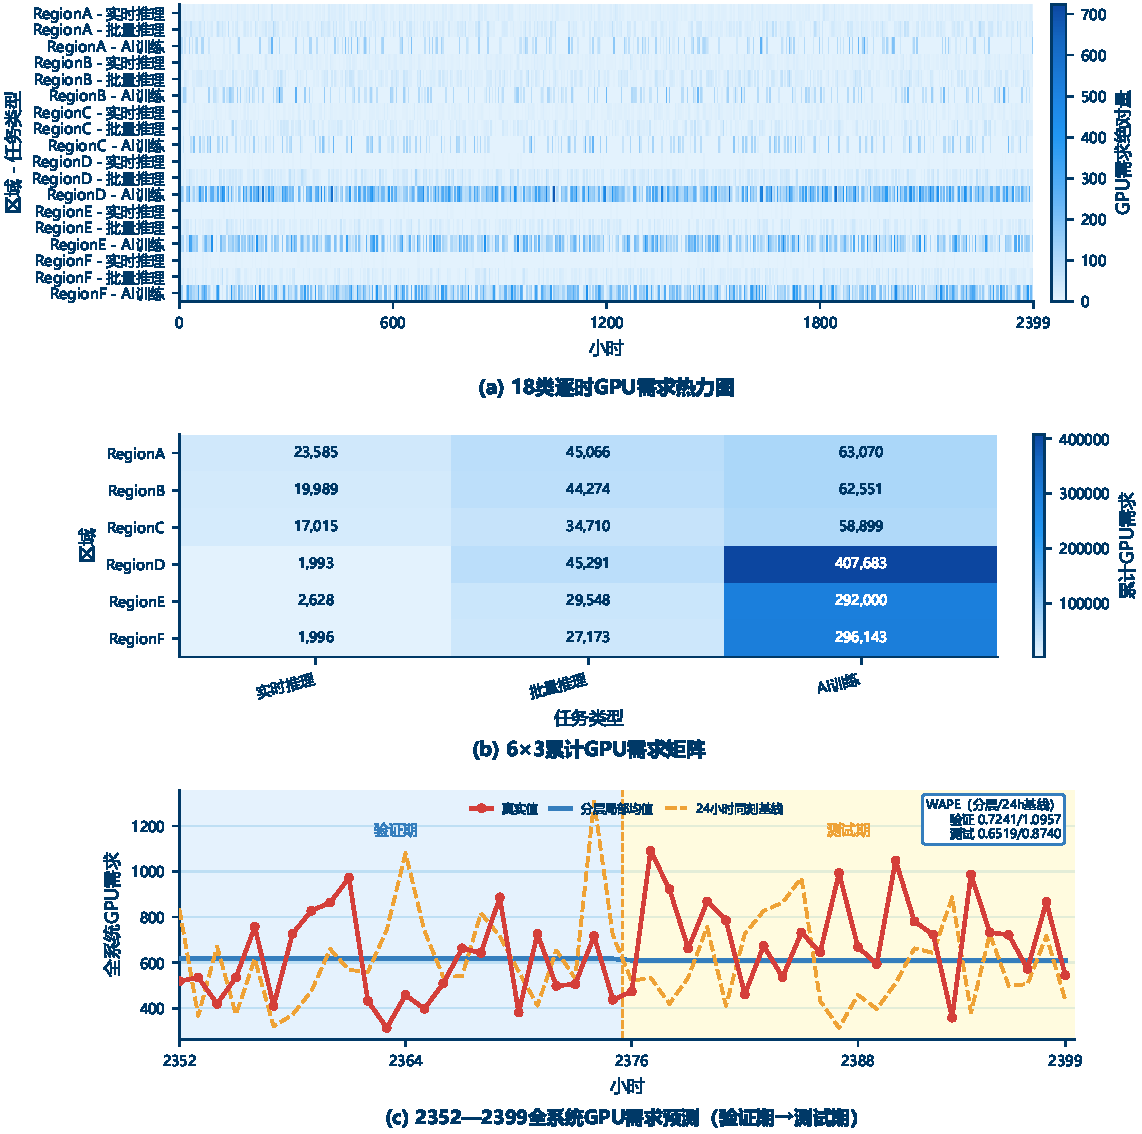
\includegraphics[width=0.88\textwidth]{figures/q1_group1_demand_structure.pdf}
%	\caption{GPU需求异质性与分层短期预测结果}
%\end{figure}
%% =================================================
%
%图1(c)进一步给出了预测结果。
%在验证期，第2352--2375小时的分层局部均值预测
%WAPE、RMSE和MAE分别为0.7241、45.7417和23.6915，
%而24小时同刻基线分别为1.0957、69.9249和35.8495；
%在测试期，第2376--2399小时对应三项指标分别为
%0.6519、53.4704和26.3323，
%基线则为0.8740、72.8628和35.3032。
%因此，在当前验证和测试划分下，
%分层局部均值模型在三项误差指标上均优于24小时同刻基线。
%从图中也可以看到，该预测更侧重于捕捉未来24小时的局部需求水平，
%而不是强行追踪难以重复的单小时尖峰。
%因此，其主要作用是稳定刻画短期总体需求水平，
%而非精确复现每一个随机峰值。
%
%完成预测后，基础算力调度直接读取第2376--2399小时实际到达的538个任务，
%预测值不参与任务安排。
%调度按照式(6)的两级目标进行：首先最小化跨区域迁移GPU工作量，
%随后在一级目标最优的条件下最小化弹性任务等待时间。
%任务实际执行过程中根据式(4)计算跨小时重叠比例，
%并结合式(5)检查GPU容量、IT功率和设施功率约束。
%
%求解结果表明，一级目标达到
%$F_1^*=0\ \mathrm{GPU\cdot h}$，
%538个任务均可在来源区域完成，本地执行率为100\%；
%在保持零迁移的条件下，二级目标得到
%$F_2^*=3\ \mathrm{h}$。
%这意味着在问题一尚未考虑电价、碳强度和新能源条件时，
%当前算力容量本身并不会迫使任务进行跨区域迁移。
%因此，后续问题二若出现任务迁移，其主要驱动力应来自能源侧条件变化，
%而不是问题一阶段的资源不可行。
%
%% ==================== 图2 ====================
%% 若整图内容较密，建议宽度用0.90--0.95\textwidth
%% 如果图片在页面上显得太高，可改为：
%% \includegraphics[width=0.90\textwidth,height=0.78\textheight,keepaspectratio]{...}
%\begin{figure}[H]
%	\centering
%	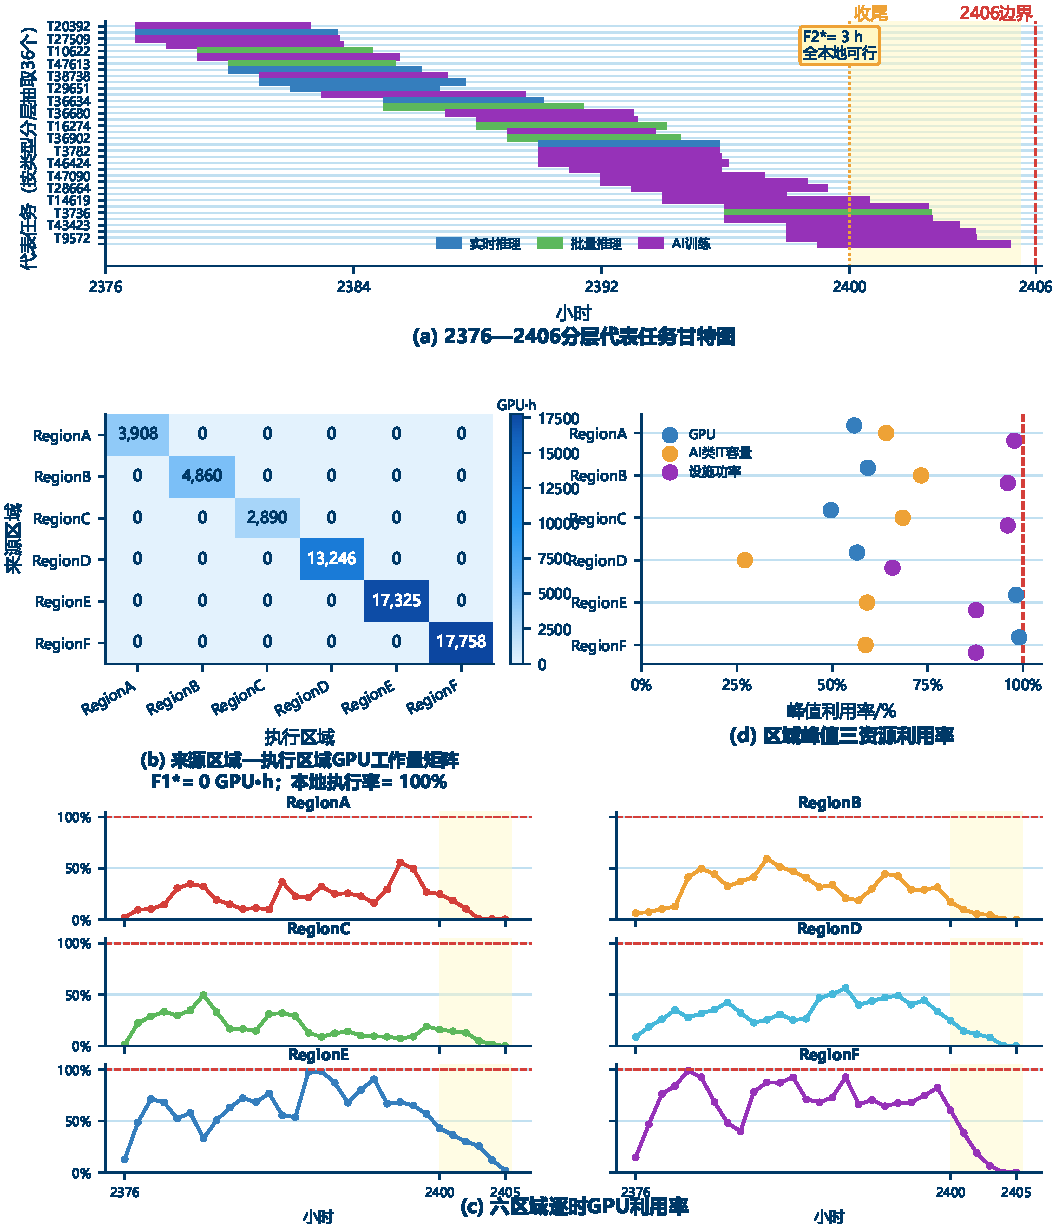
\includegraphics[width=0.92\textwidth]{figures/q1_group2_core_results.pdf}
%	\caption{基础算力调度方案与多资源承载状态}
%\end{figure}
%% =================================================
%
%图2从任务调度和资源利用两个角度进一步说明了该结果。
%代表任务甘特图显示，部分在主时域末端到达的批量推理和AI训练任务
%延伸至第2400--2405小时收尾区间，
%但所有任务均在2406边界前完成。
%来源区域--执行区域GPU工作量矩阵全部集中在主对角线上，
%与$F_1^*=0$和100\%本地执行率一致。
%
%六个区域的逐时GPU利用率进一步表明，
%不同区域的资源紧张程度并不相同。
%RegionE和RegionF在部分时段的GPU利用率接近容量上界，
%而部分东部区域虽然GPU仍有剩余，
%其设施功率利用率却已处于较高水平；
%RegionD则表现出相对充足的综合承载空间。
%因此，区域可调度能力不能仅依据GPU数量判断，
%GPU容量、AI IT功率和设施功率均可能成为实际瓶颈。
%这一结果也验证了式(5)中保留多层资源约束的必要性。
%
%为进一步检验预测结论是否依赖单一验证区间，
%对分层预测进行了84个滚动样本外窗口检验。
%如图3(a)所示，
%84个窗口中“分层模型WAPE减去24小时同刻基线WAPE”的差值全部小于0，
%即84个窗口均由分层模型取得更低WAPE，
%单侧统计检验得到$p=8.55\times10^{-16}$。
%这表明图1中观察到的预测优势并非由单一预测起点偶然产生，
%而是在不同样本外窗口中保持较稳定的一致性。
%
%同时，为检验式(3)的层级一致性恢复是否以牺牲预测精度为代价，
%将恢复后的18类需求与直接预测结果进行比较。
%图3(b)中二者WAPE中位差仅为
%$-3.05\times10^{-4}$，对应$p=0.216$，
%未观察到统计上明显的精度差异。
%另一方面，区域边际和任务类型边际的最大闭合误差均为
%$6.82\times10^{-13}$，
%18类汇总误差为$4.11\times10^{-10}$。
%因此，层级恢复的主要作用是保证区域、任务类型和系统总量之间的逻辑一致，
%而不是通过人为调整改善误差指标。
%
%% ==================== 图3 ====================
%% 检验图通常信息较密，可以稍微放大
%% 如果图片总是被LaTeX推到下一页，可尝试把[htbp]改成[!htbp]
%% 若仍不理想，可在图前加 \clearpage，但不建议频繁使用
%\begin{figure}[H]
%	\centering
%	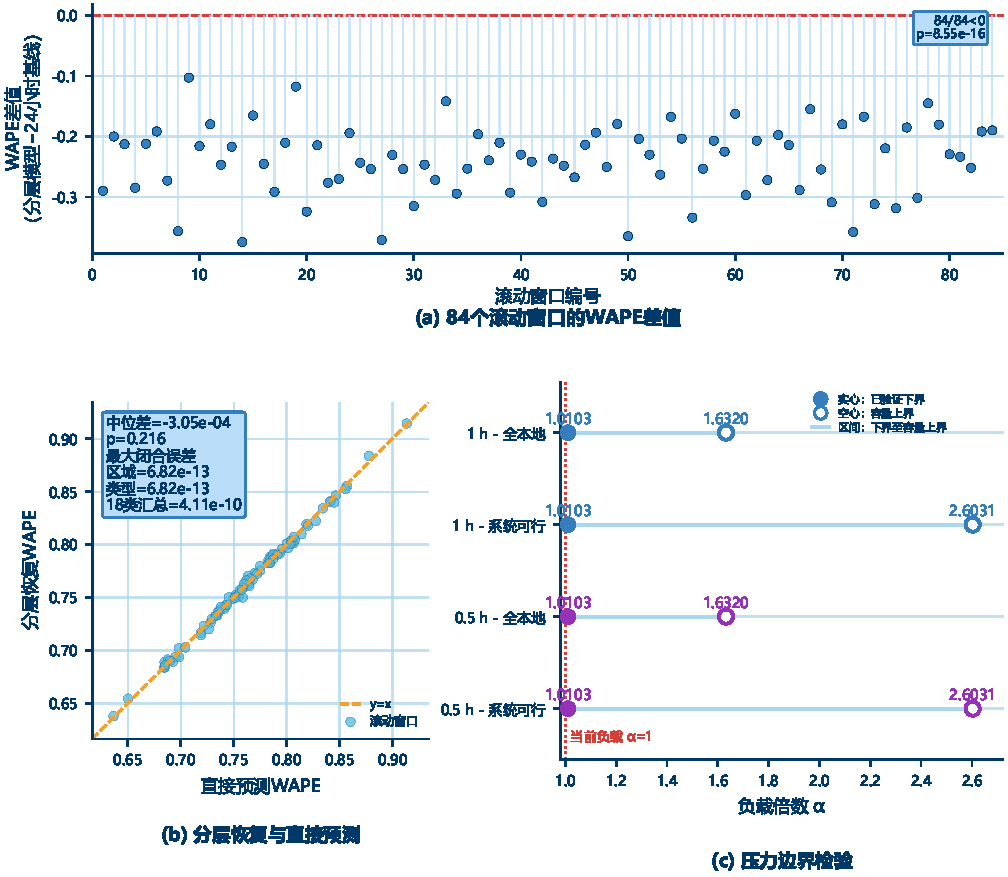
\includegraphics[width=0.91\textwidth]{figures/q1_group3_validation_robustness.pdf}
%	\caption{分层预测稳定性与算力调度压力边界检验}
%\end{figure}
%% =================================================
%
%除预测稳定性外，还对基础调度的资源边界进行了压力检验。
%设原始任务负荷按照比例系数$\alpha$整体放大，
%当前运行点对应$\alpha=1$。
%图3(c)表明，已经实际验证可行的负载下界为$\alpha=1.0103$；
%在容量关系下，保持全本地运行的上界为1.6320，
%允许跨区域协调后的系统容量上界为2.6031。
%需要强调的是，1.6320和2.6031仅表示由资源容量关系得到的上界，
%并不能直接解释为已经验证可行的精确临界负载。
%因此，该压力测试更准确地给出了
%“已验证可行负荷”与“理论容量上限”之间的边界区间。
%
%此外，为检验整数小时开工假设是否影响核心调度结论，
%进一步采用0.5小时粒度重新求解。
%1小时和0.5小时两种粒度下均得到
%$F_1^*=0$，
%说明“当前任务无需跨区域迁移”这一一级结论保持不变；
%累计弹性等待时间则由3 h下降至2 h，
%表明时间粒度细化主要改善少量任务的局部开工安排，
%并未改变整体空间调度判断。
%与此同时，对任务唯一执行、实时任务立即启动、网络时延、
%最早开工、最晚完成、2406终端边界以及GPU、IT功率和设施功率等硬约束进行复核，
%均未发现约束违反。
%
%综合上述结果，
%问题一的分层预测能够在保留区域与任务类型异质性的同时，
%稳定提取短期GPU需求水平；
%层级一致性恢复在几乎不改变预测精度的情况下保证了多层需求闭合。
%基础算力调度则表明，
%当前任务规模下六区域已有资源能够支持全部任务本地完成，
%但不同区域的GPU、AI IT功率和设施功率瓶颈存在明显差异。
%这些结果为后续碳感知调度提供了明确基线：
%后续产生的跨区域迁移应主要反映电价、碳强度和新能源条件所带来的算电协同效应。
%
\section{问题一的模型建立与求解}

\subsection{数据预处理}

原始数据含50000个任务、6个区域和3类任务，到达时刻覆盖第0--2399小时。检查字段完整性与取值范围后，将持续时间由分钟换算为小时，按任务类型匹配单位GPU功率，并按最大网络时延筛选候选区域；各物理量不作标准化或异常值删除。预测数据按“到达小时--来源区域--任务类型”聚合并补齐零需求，共43200条记录；第0--2351小时用于训练，第2352--2375小时用于验证，第2376--2399小时用于测试。调度直接采用测试期实际任务，第2400--2405小时用于收尾，第2406小时为终端边界。


\subsection{模型建立}

问题一分别进行GPU需求短期预测与基础算力调度，预测结果仅用于精度评价，不参与实际调度。

设区域$r$、任务类型$k$在时刻$t$的新到达GPU需求为$D_{rkt}$，
任务$i$的GPU需求为$g_i$，则
\begin{equation}
	D_{rkt}
	=
	\sum_{\substack{i:\,a_i=t\\
			r_i^0=r,\;k(i)=k}}
	g_i .
	\label{eq:q1_demand}
\end{equation}

由此得到18条底层序列，并构造区域需求$D_{rt}=\sum_kD_{rkt}$、任务类型需求$D_{kt}=\sum_rD_{rkt}$和系统需求$D_t=\sum_rD_{rt}$。底层序列保留异质性，三个聚合层用于提高短期预测稳定性。

层级与分组时间序列需通过预测协调保持层间一致\cite{ref4}。本文以历史业务占比构造非负先验，采用广义KL散度恢复18类交叉需求，借鉴一致性恢复思想而不直接使用Trace MinT目标函数。

对于任一聚合需求序列$y_t$，
采用预测时点前最近$H$小时的平均需求水平预测未来24小时：
\begin{equation}
	\hat{y}_{T+h}(H)
	=
	\frac{1}{H}
	\sum_{\tau=T-H+1}^{T}y_{\tau},
	\qquad h=1,2,\ldots,24 .
	\label{eq:q1_localmean}
\end{equation}

其中$T$为预测前最后一个已知时刻。由验证集在$H\in\{24,72,168,336\}$中选窗，再用第0--2375小时信息预测第2376--2399小时，测试期不参与模型选择。

区域、任务类型和系统需求分别预测后可能出现总量不一致，
因此首先以系统预测$\hat D_t^{(S)}$作为总量锚点，
对区域和任务类型边际进行比例校正，
得到$\tilde D_{rt}$和$\tilde D_{kt}$。
设历史区域--任务类型平均需求占比为$q_{rk}$，
构造与GPU需求同量纲的先验
$q^0_{rkt}=q_{rk}\hat D_t^{(S)}$；
对于历史占比为0的组合赋予极小正数以避免对数奇异。
随后利用广义KL散度恢复18类交叉需求：
\begin{equation}
	\begin{aligned}
		\min_{z_{rkt}\geq0}\quad
		&\sum_r\sum_k
		\left[
		z_{rkt}\ln\frac{z_{rkt}}{q^0_{rkt}}
		-z_{rkt}+q^0_{rkt}
		\right],\\
		\mathrm{s.t.}\quad
		&\sum_kz_{rkt}=\tilde D_{rt},\\
		&\sum_rz_{rkt}=\tilde D_{kt}.
	\end{aligned}
	\label{eq:q1_kl}
\end{equation}

式(\ref{eq:q1_kl})在保持两类边际不变时使18类需求接近历史结构。预测采用WAPE、RMSE和MAE评价，以24小时前同刻需求为基准。

基础算力调度直接采用第2376--2399小时实际到达任务。
设任务$i$持续时间为$d_i$、来源区域为$r_i^0$，
根据网络时延确定候选区域$R_i$。
实时推理任务到达即开工；
批量推理和AI训练任务在最早开工时间、最晚完成时间及2406终端边界内确定候选开工集合$S_i$。
定义$x_{irs}$表示任务$i$是否在区域$r$、时刻$s$开工。

由于任务持续时间保留分钟精度，而资源容量按小时统计，
定义任务$i$从时刻$s$开始后与小时区间$[t,t+1)$的实际运行比例为
\begin{equation}
	\rho_{ist}
	=
	\max\left\{
	0,\,
	\min(s+d_i,t+1)-\max(s,t)
	\right\}.
	\label{eq:q1_overlap}
\end{equation}

由式(\ref{eq:q1_overlap})可计算逐小时GPU和功率占用。
任务$i$完整运行时的AI IT功率为
$p_i=g_iP^{GPU}_{k(i)}$。
区域$r$在时刻$t$可供AI任务使用的有效IT功率定义为
\[
A_{rt}
=
\max\left\{
0,\,
\min\left(
P^{IT,\max}_r-P^{NonAI}_{rt},
\frac{P^{Facility,\max}_r}{PUE_r}-P^{NonAI}_{rt}
\right)
\right\}.
\]
主要资源约束为
\begin{equation}
	\begin{aligned}
		&\sum_{r\in R_i}\sum_{s\in S_i}x_{irs}=1,
		&&\forall i,\\
		&\sum_i\sum_{s\in S_i}
		g_i\rho_{ist}x_{irs}
		\leq G^{ava}_{rt},
		&&\forall r,t,\\
		&\sum_i\sum_{s\in S_i}
		p_i\rho_{ist}x_{irs}
		\leq A_{rt},
		&&\forall r,t .
	\end{aligned}
	\label{eq:q1_capacity}
\end{equation}

式(\ref{eq:q1_capacity})保证任务唯一执行及GPU、功率容量可行；$R_i$和$S_i$预先筛除违反时延、时窗或终端边界的组合。

问题一不引入电价、碳排放、新能源和储能因素，
因此作为后续算电协同调度的中性算力基线。
首先最小化跨区域迁移GPU工作量，
再在一级目标最优的条件下最小化弹性任务累计等待时间：
\begin{equation}
	\begin{aligned}
		\min\quad
		F_1
		&=
		\sum_i
		\sum_{\substack{r\in R_i\\r\neq r_i^0}}
		\sum_{s\in S_i}
		g_id_ix_{irs},\\
		\text{在 }F_1=F_1^{*}\text{ 条件下，}\qquad
		\min\quad
		F_2
		&=
		\sum_{i\in I^{\mathrm{flex}}}
		\sum_{r\in R_i}\sum_{s\in S_i}
		(s-e_i)x_{irs}.
	\end{aligned}
	\label{eq:q1_objective}
\end{equation}

其中$F_1$衡量迁移GPU工作量，$F_2$为弹性任务累计等待时间。


\subsection{求解结果与模型检验}

验证集中$H=72$的总体WAPE最低，据此用第0--2375小时历史数据预测第2376--2399小时的18类GPU需求。

RegionD、RegionE和RegionF的AI训练累计GPU需求分别为
407683、292000和296143，
明显高于RegionA、RegionB和RegionC的
63070、62551和58899；
同时底层小时需求存在较多低值和随机尖峰，
说明直接预测18条细粒度序列容易受到随机任务到达影响。

% ==================== Q1：预测误差对比 ====================
\begin{table}[H]
	\centering
	\caption{分层预测模型与24小时同刻基准误差对比}
	\label{tab:q1_forecast}
	
	\fontsize{10.5pt}{12pt}\selectfont
	\renewcommand{\arraystretch}{0.88}
	
	\begin{tabular}{ccccccc}
		\toprule
		\multirow{2}{*}{\textbf{阶段}}
		& \multicolumn{3}{c}{\textbf{分层局部均值预测}}
		& \multicolumn{3}{c}{\textbf{24小时同刻基准}}\\
		\cmidrule(lr){2-4}\cmidrule(lr){5-7}
		& \textbf{WAPE} & \textbf{RMSE} & \textbf{MAE}
		& \textbf{WAPE} & \textbf{RMSE} & \textbf{MAE}\\
		\midrule
		验证期
		& 0.7241 & 45.7417 & 23.6915
		& 1.0957 & 69.9249 & 35.8495\\
		
		测试期
		& 0.6519 & 53.4704 & 26.3323
		& 0.8740 & 72.8628 & 35.3032\\
		\bottomrule
	\end{tabular}
\end{table}


表\ref{tab:q1_forecast}中，分层模型在验证期和测试期的三项误差均低于24小时同刻基准。题面分别要求短期需求预测和末段基础算力调度，因此预测结果用于评价需求变化的可预测程度，实际调度仍以第2376--2399小时真实到达的任务为输入，避免预测误差改变任务级可行性。验证期与测试期的WAPE分别为0.7241和0.6519，表明稀疏需求和随机尖峰仍较难准确刻画。测试期WAPE降低而RMSE升高并不矛盾：WAPE按总实际需求归一化，RMSE则对少数较大误差更加敏感，二者反映了不同的误差特征。

\begin{figure}[H]
	\centering
	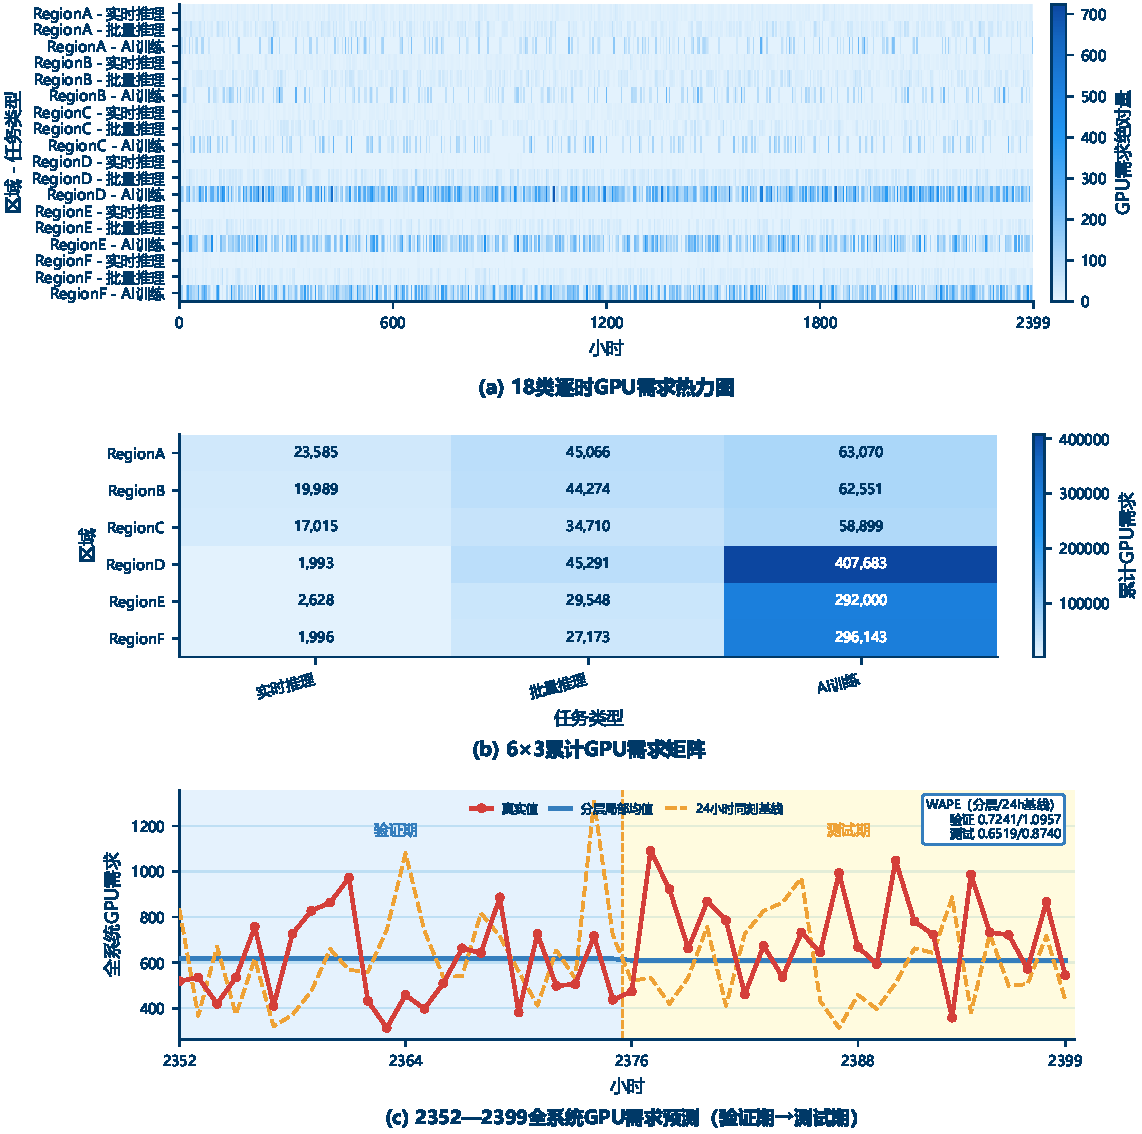
\includegraphics[width=0.80\textwidth]{figures/q1_group1_demand_structure.pdf}
	\caption{GPU需求异质性与分层短期预测结果}
	\label{fig:q1_forecast}
\end{figure}

图\ref{fig:q1_forecast}显示模型主要刻画短期需求水平，不追踪随机单小时尖峰。

基础调度对第2376--2399小时实际到达的538个任务按式(\ref{eq:q1_objective})进行两级优化。

% ==================== Q1：基础调度结果 ====================
\begin{table}[H]
	\centering
	\caption{基础算力调度优化结果}
	\label{tab:q1_dispatch}
	
	\fontsize{10.5pt}{12pt}\selectfont
	\renewcommand{\arraystretch}{0.88}
	
	\begin{tabular}{cc}
		\toprule
		\textbf{评价指标} & \textbf{优化结果}\\
		\midrule
		任务数量 & 538\\
		一级目标$F_1^*$ & $0$ GPU$\cdot$h\\
		本地执行率 & 100\%\\
		二级目标$F_2^*$ & 3 h\\
		求解相对间隙 & 0\\
		\bottomrule
	\end{tabular}
\end{table}


表\ref{tab:q1_dispatch}中$F_1^*=0$、$F_2^*=3$ h，538个任务均可在来源区域完成，当前资源下无须迁移即可保证可行。

\begin{figure}[H]
	\centering
	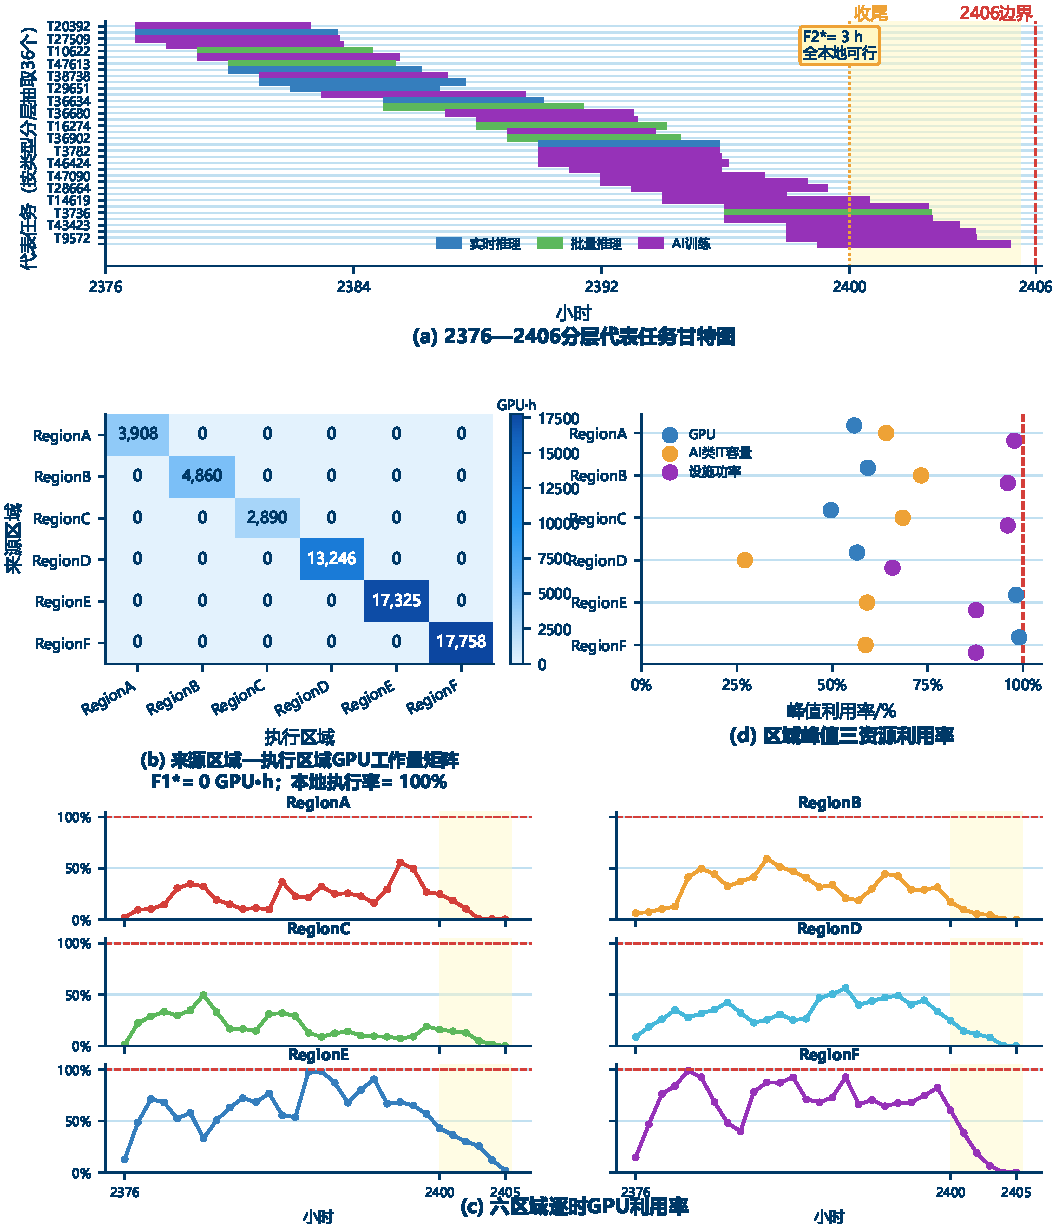
\includegraphics[width=0.75\textwidth]{figures/q1_group2_core_results.pdf}
	\caption{基础算力调度方案与多资源承载状态}
	\label{fig:q1_dispatch}
\end{figure}

图\ref{fig:q1_dispatch}显示，末端任务均在2406前完成，区域间GPU工作量矩阵仅主对角线非零；RegionE、RegionF部分时段接近GPU容量边界，部分东部区域受设施功率限制。

84个滚动样本外窗口中，分层模型WAPE均低于24小时同刻基准；单侧Wilcoxon检验得$p=8.55\times10^{-16}$。

一致性恢复与直接预测的WAPE中位差为$-3.05\times10^{-4}$（$p=0.216$），区域、类型边际最大闭合误差均为$6.82\times10^{-13}$，18类汇总误差为$4.11\times10^{-10}$。其作用是保证多层预测闭合，而非提高精度。

\begin{figure}[H]
	\centering
	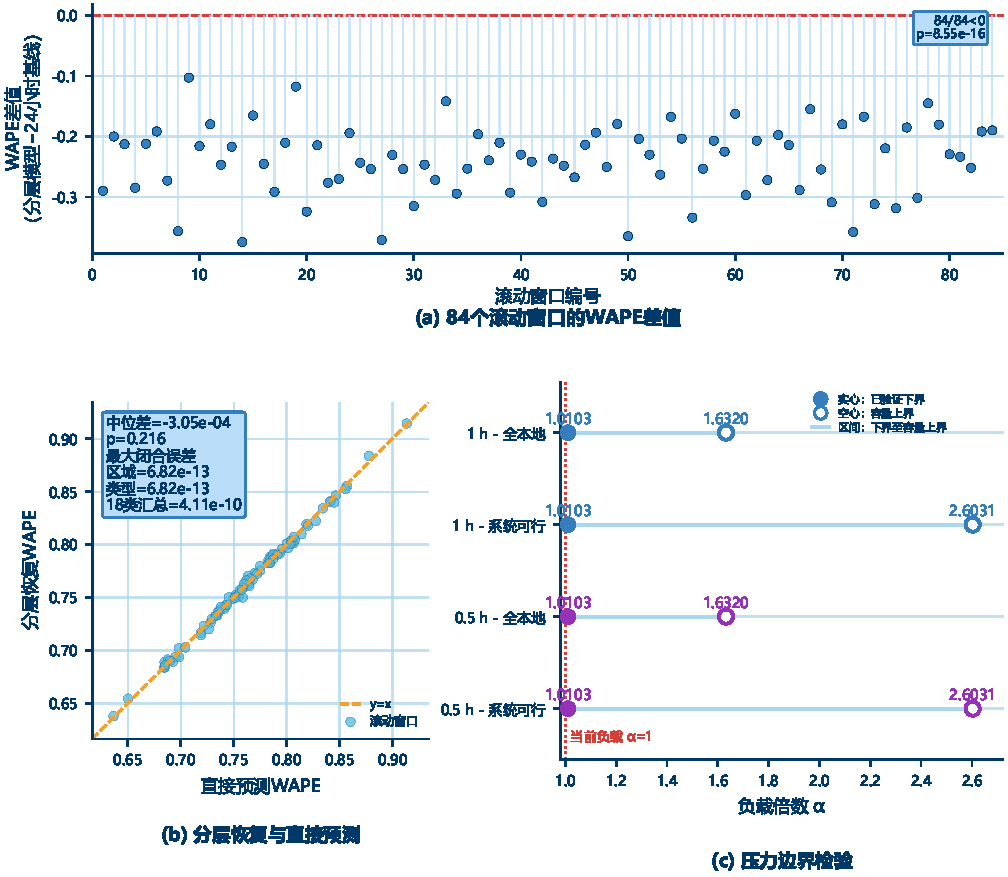
\includegraphics[width=0.80\textwidth]{figures/q1_group3_validation_robustness.pdf}
	\caption{分层预测稳定性与算力调度压力边界检验}
	\label{fig:q1_validation}
\end{figure}

图\ref{fig:q1_validation}中，负荷放大系数$\alpha$的已验证可行下界为1.0103；全本地和跨区域协调的容量理论上界分别为1.6320、2.6031，后两者并非已验证的精确临界值。

0.5小时粒度复算仍有$F_1^*=0$，累计等待由3 h降至2 h，未改变无需迁移的结论；任务唯一执行、实时启动、时延、时限及各容量约束均未发现违反。

问题一由此形成短期需求预测和纯算力调度基准，供问题二引入能源因素后比较。



	\section{问题二的模型建立与求解}

\subsection{模型建立}

问题二使用第0--2399小时实际任务和逐时电力参数重新优化执行区域与开工时刻，预测结果不参与调度；第2400--2405小时仅用于收尾和结算，任务须在2406前完成。本问不考虑储能。
碳感知数据中心研究表明，电力碳强度可以作为任务调度和能源管理的重要决策信号\cite{ref5}；
跨区域负荷迁移能够利用不同区域的电力与碳排放差异，
但同时会引入网络时延和服务质量代价\cite{ref6}。
据此在任务时限、网络时延、GPU及功率约束下评价成本、碳排放、通信时延和新能源利用率。

任务参数及跨小时占用沿用问题一；实时任务立即开工，弹性任务可在合法时窗内错峰。
设$x_{irs}$表示任务$i$是否在区域$r$、时刻$s$开工，
候选区域$R_i$满足网络时延限制，
候选开工集合$S_i$满足到达时间、完成期限及2406终端约束。

设区域$r$在时刻$t$的AI IT负荷、总IT负荷和设施负荷分别为
$P^{AI}_{rt}$、$P^{IT}_{rt}$和$F_{rt}$。
利用问题一式(\ref{eq:q1_overlap})中的跨小时占用比例，有
\begin{equation}
	\begin{aligned}
		P^{AI}_{rt}
		&=
		\sum_i\sum_{s\in S_i}
		p_i\rho_{ist}x_{irs},\\
		P^{IT}_{rt}
		&=
		P^{NonAI}_{rt}+P^{AI}_{rt},\\
		F_{rt}
		&=
		PUE_rP^{IT}_{rt}.
	\end{aligned}
	\label{eq:q2_load_mapping}
\end{equation}

逐时GPU占用仍满足问题一约束。将IT容量、设施容量和最大购电能力合并为有效AI IT容量
$\bar P^{AI}_{rt}
=\min\{P^{IT,\max}_{rt}-P^{NonAI}_{rt},
P^{Facility,\max}_{rt}/PUE_r-P^{NonAI}_{rt},
(P^{RE}_{rt}+P_r^{Grid,\max})/PUE_r-P^{NonAI}_{rt}\}$，
并要求$P^{AI}_{rt}\leq\bar P^{AI}_{rt}$；其余GPU、时延和时限约束沿用问题一。

无储能时，新能源优先供给本地负荷，不足由电网补充，富余部分按上限外送，其余弃用。
设$V_{rt}$、$B_{rt}$、$X_{rt}$和$R_{rt}$分别为
新能源直接消纳、电网购电、新能源外送和弃用功率，则
\begin{equation}
	\begin{aligned}
		V_{rt}&=\min(F_{rt},P^{RE}_{rt}),\\
		B_{rt}&=\max(F_{rt}-P^{RE}_{rt},0),\\
		X_{rt}&=\min\{\max(P^{RE}_{rt}-F_{rt},0),\bar X_r\},\\
		R_{rt}&=P^{RE}_{rt}-V_{rt}-X_{rt},
	\end{aligned}
	\label{eq:q2_energy}
\end{equation}
其中$0\leq B_{rt}\leq P_r^{Grid,\max}$，$0\leq X_{rt}\leq\bar X_r$。

以净运行成本$C$、碳排放$E$、平均网络时延$L$
和新能源利用率$U$评价方案。
在$t=0,\ldots,2405$上定义
\begin{equation}
	\begin{aligned}
		C
		&=
		\sum_r\sum_{t=0}^{2405}
		\left(\pi_{rt}B_{rt}-\sigma_{rt}X_{rt}\right),\\
		E
		&=
		\sum_r\sum_{t=0}^{2405}\kappa_{rt}B_{rt},\\
		L
		&=
		\frac{1}{N}
		\sum_i\sum_{r\in R_i}\sum_{s\in S_i}
		l_{ir}x_{irs},\\
		U
		&=
		\frac{\displaystyle
			\sum_r\sum_{t=0}^{2405}(V_{rt}+X_{rt})}
		{\displaystyle
			\sum_r\sum_{t=0}^{2405}P^{RE}_{rt}},
		\qquad Q=1-U.
	\end{aligned}
	\label{eq:q2_objectives}
\end{equation}

令$f_1=C,f_2=E,f_3=L,f_4=Q$。分别求解单目标连续松弛得到理想下界$f_m^{LB}$，再结合纯算力基准$f_m^0$和单目标锚点$x^{(a)}$建立固定尺度：
\begin{equation}
	\begin{aligned}
		f_m^{ref}
		&=
		\max\left\{
		f_m^0,\max_a f_m(x^{(a)})
		\right\},\\
		R_m
		&=
		f_m^{ref}-f_m^{LB},\\
		d_m(x)
		&=
		\frac{f_m(x)-f_m^{LB}}{R_m},\\
		\min\quad z,
		&\qquad d_m(x)\leq z,\quad \forall m .
	\end{aligned}
	\label{eq:q2_minmax}
\end{equation}

若$R_m\approx0$，该指标仅用于结果评价；否则式(\ref{eq:q2_minmax})最小化最大标准化偏离。

多时间尺度滚动常用于处理任务到达、负荷和能源状态的动态耦合\cite{ref7}，低碳在线调度还需协调服务质量与能源指标\cite{ref8}。针对50000个任务，本文采用$H=24$ h决策窗口、$K=48$ h前瞻窗口，结合可行性修复和局部混合整数线性规划精修。
在滚动起点$\tau$，
考察$[\tau,\tau+H+K)$范围，
但仅固定$[\tau,\tau+H)$内实际开工任务；
已开工任务保持原安排，
最晚合法开工时刻进入当前窗口的弹性任务必须在本轮开工。

构造阶段先安排实时任务，再按时间裕量和资源需求排序处理弹性任务。
定义当前全时域目标估计
$\hat f_{m,\tau}
=f_m^0+\Delta f_{m,\tau}^{past}
+f_{m,\tau}^{scope}-f_{m,\tau}^{0,scope}$。
对合法候选$(r,s)$计算
\begin{equation}
	S_{irs}
	=
	\max_m
	\left\{
	\frac{
		\hat f_{m,\tau}
		+\Delta f_{m,irs}
		-f_m^{LB}}
	{R_m}
	\right\},
	\qquad
	(r_i^*,s_i^*)
	=
	\arg\min_{(r,s)}S_{irs}.
	\label{eq:q2_marginal}
\end{equation}

若出现容量冲突则重排可替代任务；得到可行解后选择关键任务形成大邻域，并固定邻域外决策进行精修，流程见表\ref{tab:q2_algorithm}。

\begin{table}[H]
	\centering
	\caption{问题二滚动数学启发式求解流程}
	\label{tab:q2_algorithm}
	
	\fontsize{10.5pt}{12pt}\selectfont
	\renewcommand{\arraystretch}{0.88}
	
	\begin{tabular}{
			>{\centering\arraybackslash}p{0.08\textwidth}
			>{\raggedright\arraybackslash}p{0.86\textwidth}}
		\toprule
		\textbf{步骤} & \multicolumn{1}{c}{\textbf{主要操作}}\\
		\midrule
		
		1 &
		由连续松弛、问题二纯算力基准及单目标锚点确定固定定标尺度。\\
		
		2 &
		读取$H=24$ h决策窗口与$K=48$ h前瞻区，
		锁定已开工任务并识别本轮必须开工任务。\\
		
		3 &
		实时任务立即安排；弹性任务按时间裕量和资源需求排序，
		利用式(\ref{eq:q2_marginal})选择可行候选。\\
		
		4 &
		更新GPU、AI IT负荷和能源状态；
		出现容量冲突时重新安排可替代任务。\\
		
		5 &
		选择关键任务形成大邻域，
		固定邻域外方案并利用小规模混合整数线性规划模型精修。\\
		
		6 &
		提交当前$H$小时决策并继续滚动；
		最终重构0--2405小时全时域剖面并独立核验。\\
		
		\bottomrule
	\end{tabular}
\end{table}


该方法按原多目标准则评价候选，数学启发式仅缩小整数搜索范围；所得结果为严格满足硬约束且计算效率较高的可行方案，不宣称获得全局最优解。


\subsection{求解结果与模型检验}

按问题一原则构造50000个任务的全时域纯算力基准，并以问题二能源口径结算；滚动求解结果见表\ref{tab:q2_result}。

% ==================== Q2：多目标结果 ====================
\begin{table}[H]
	\centering
	\caption{问题二多目标调度与问题二纯算力基准对比}
	\label{tab:q2_result}
	
	\fontsize{10.5pt}{12pt}\selectfont
	\renewcommand{\arraystretch}{0.90}
	
	\begin{tabular}{lccc}
		\toprule
		\multicolumn{1}{c}{\textbf{评价指标}}
		& \textbf{问题二纯算力基准}
		& \textbf{问题二均衡方案}
		& \textbf{变化}\\
		\midrule
		
		净运行成本/元
		& $-4.196834\times10^8$
		& $-4.247568\times10^8$
		& 降低507.34万元\\
		
		碳排放/tCO$_2$
		& 8.850562
		& 10.125791
		& 增加1.275228\\
		
		平均网络时延/ms
		& 5.000000
		& 12.946840
		& 增加7.946840\\
		
		新能源利用率
		& 67.91598\%
		& 68.13914\%
		& 提高0.22316个百分点\\
		
		平均等待时间/h
		& 0.00116
		& 30.89284
		& 增加30.89168\\
		
		跨区域迁移比例
		& 0
		& 29.35800\%
		& 增加29.35800个百分点\\
		
		\bottomrule
	\end{tabular}
\end{table}


表\ref{tab:q2_result}显示，净运行成本降低507.34万元、新能源利用率提高0.22316个百分点，但碳排放增加1.2752 tCO$_2$、平均网络时延增加7.95 ms；负成本表示外送收益超过购电支出。

固定定标后，纯算力基准四项偏离为1.00、1.00、0和1.00，问题二方案为0.85、1.14、1.15和0.87，最大偏离$z=1.15$。

\begin{figure}[H]
	\centering
	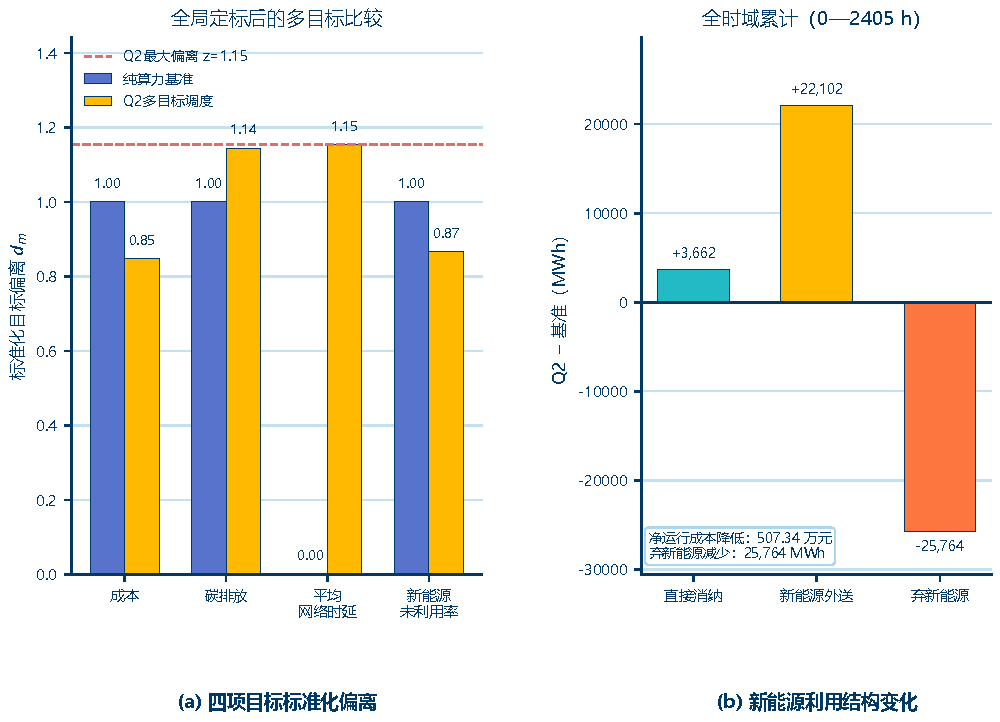
\includegraphics[width=0.82\textwidth]
	{figures/q2_group1_core_results.pdf}
	\caption{问题二多目标调度效果及新能源利用结构变化}
	\label{fig:q2_core}
\end{figure}

图\ref{fig:q2_core}中，新能源直接消纳、外送分别增加约3662、22102 MWh，弃用减少约25764 MWh，变化量基本闭合。

共有35321个任务本地执行、14679个跨区域迁移，迁移比例29.358\%，迁移GPU工作量为$1.308142\times10^6\,\mathrm{GPU\cdot h}$。

图\ref{fig:q2_migration}显示D、E、F迁出较多，C、D吸收较多跨区域算力，迁移方向同时受资源和能源条件影响。

依据50000条任务记录重构0--2405小时剖面，两方案累计量保持一致：AI IT能耗均为$7.389279853\times10^5$ MWh，GPU工作量均为$5.020787\times10^6$ GPU$\cdot$h；
任务、时延、时限、容量和购电边界均无违反，能源平衡残差为0，2406时点无任务占用。

91个精修窗口中45个接受改进，平均改善2.43\%。窗口0--9的同窗精确对照显示，中位计算速度提高约31.8倍，平均绝对相对偏差为39.82\%，最大标准化目标偏差为293.40\%。该最大值是局部窗口标准化目标的相对偏差，不等同于全时域成本、碳排放等指标的整体误差，但表明受限邻域在个别资源紧张窗口中可能遗漏更优的任务组合。因此，本文仅将其作为能够严格满足硬约束的大规模近似求解方法，不宣称获得局部或全时域最优解。

\begin{figure}[H]
	\centering
	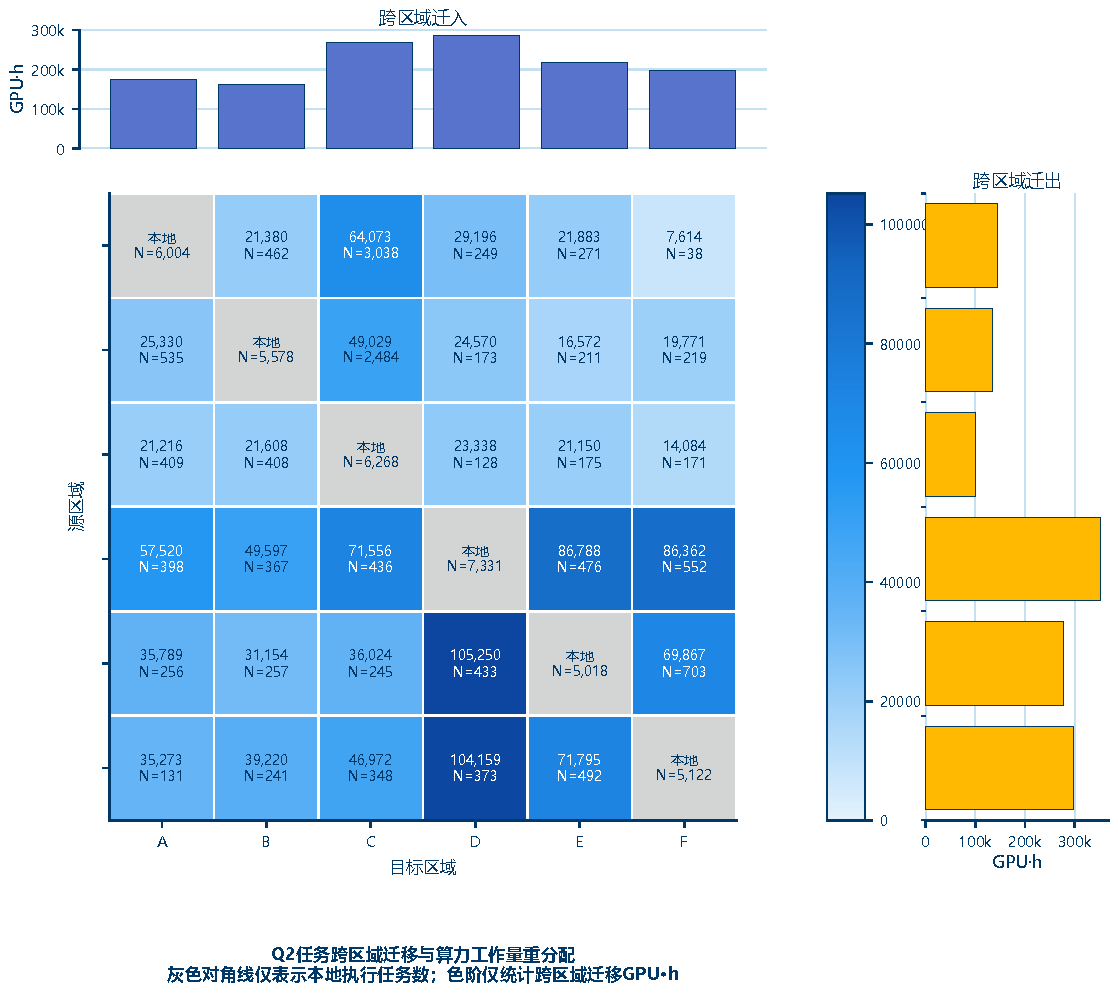
\includegraphics[width=0.68\textwidth]
	{figures/q2_group2_dispatch_mechanism.pdf}
	\caption{问题二任务跨区域迁移与算力工作量重分配}
	\label{fig:q2_migration}
\end{figure}

\begin{figure}[H]
	\centering
	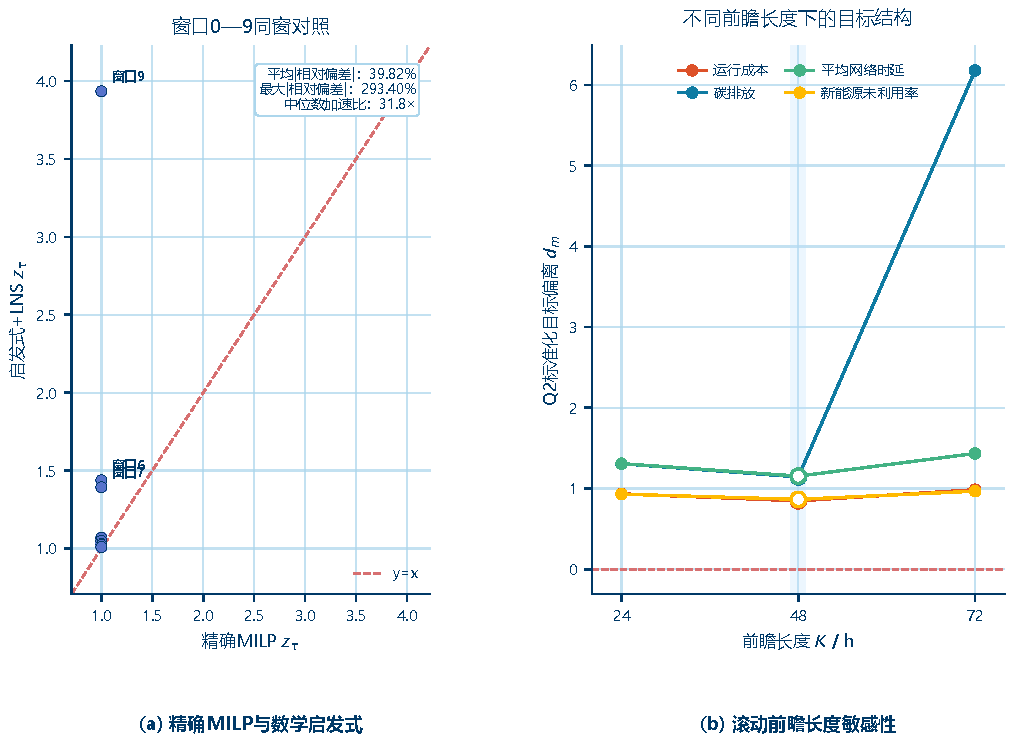
\includegraphics[width=0.72\textwidth]
	{figures/q2_group3_model_validation.pdf}
	\caption{问题二数学启发式求解质量与前瞻长度敏感性}
	\label{fig:q2_validation}
\end{figure}

前瞻长度检验中，$K=24$ h与48 h的目标结构接近，$K=72$ h仅使碳排放明显增大，故采用$H=24$ h、$K=48$ h。

问题二以碳排放、网络时延和等待增加换取成本降低与新能源利用提高，全时域复算满足硬约束，可作为问题四任务侧初始方案。

	\section{问题三的模型建立与求解}

\subsection{模型建立}

问题三固定题目给定的AI与非AI IT负荷，不调整任务区域和开工时刻，仅优化新能源分配、储能充放电及购售电，以识别储能的能源侧作用。

设区域$r$在时段$t$的设施负荷为$F_{rt}$，
可用新能源功率为$P^{RE}_{rt}$，
电网购电功率为$B_{rt}$；
新能源直接供能、新能源充电、电网充电、储能放电、
新能源外送和弃用功率分别记为
$V_{rt}$、$C^{RE}_{rt}$、$C^G_{rt}$、
$D_{rt}$、$X_{rt}$和$R_{rt}$。
设施负荷与逐时能源平衡满足
\begin{equation}
	\begin{aligned}
		F_{rt}
		&=
		PUE_r
		\left(
		P^{AI}_{rt}+P^{NonAI}_{rt}
		\right),\\
		P^{RE}_{rt}
		&=
		V_{rt}+C^{RE}_{rt}+X_{rt}+R_{rt},\\
		B_{rt}+V_{rt}+D_{rt}
		&=
		F_{rt}+C^G_{rt}.
	\end{aligned}
	\label{eq:q3_energy_balance}
\end{equation}

其中$F_{rt}$已知，且$0\leq V_{rt}\leq F_{rt}$、$0\leq C^G_{rt}\leq B_{rt}$。

设$S_{rt}$为时段$t$开始时的储能电量。数据中心储能调度通常依据SOC递推和功率边界实现跨时调节\cite{ref10}；本文进一步加入充放电互斥、购售电边界和终端SOC约束，进行全时域求解。
时间步长为1 h，充、放电效率分别为$\eta_r^c$和$\eta_r^d$，
则SOC递推为
\begin{equation}
	S_{r,t+1}
	=
	S_{rt}
	+
	\eta_r^c
	\left(
	C^{RE}_{rt}+C^G_{rt}
	\right)
	-
	\frac{D_{rt}}{\eta_r^d}.
	\label{eq:q3_soc}
\end{equation}

储能满足容量、功率及$S_{r,2406}\geq S_{r0}$；引入$y_{rt}\in\{0,1\}$排除同时充放电：
$C^{RE}_{rt}+C^G_{rt}\leq y_{rt}P_r^{ch,\max}$、
$D_{rt}\leq(1-y_{rt})P_r^{dis,\max}$。
购电满足$0\leq B_{rt}\leq P_r^{Grid,\max}$；新能源外送满足$0\leq X_{rt}\leq\bar X_r$及$X_{rt}\leq P_r^{Grid,\mathrm{out},\max}$。

沿用问题二的成本和碳排放口径，并增加峰值净购电与净购电波动指标。
定义区域净购电功率$N_{rt}=B_{rt}-X_{rt}$，
则
\begin{equation}
	\begin{aligned}
		C&=
		\sum_r\sum_t
		\left(
		\pi_{rt}B_{rt}-\sigma_{rt}X_{rt}
		\right),\\
		E&=
		\sum_r\sum_t
		\kappa_{rt}B_{rt},\\
		P&=
		\sum_rP_r^{\max},
		\qquad
		P_r^{\max}\geq N_{rt},\quad
		P_r^{\max}\geq0,\\
		W&=
		\frac{1}{6(T-1)}
		\sum_r\sum_tW_{rt}.
	\end{aligned}
	\label{eq:q3_objectives}
\end{equation}

其中$t=0,\ldots,2405$，$T=2406$；$W_{rt}\geq\pm(N_{r,t+1}-N_{rt})$，故$W$为相邻小时净购电的平均绝对变化量，$P_r^{\max}\geq0$避免将净外送解释为负峰值。

四项指标量纲不同且无给定权重，先求单目标理想值$f_m^{best}$，再将各单目标方案$x^{(j)}$代入全部指标，取$f_m^{ref}=\max_j f_m(x^{(j)})$。
对于存在有效权衡关系的指标，定义
\begin{equation}
	\bar f_m
	=
	\frac{f_m-f_m^{best}}
	{f_m^{ref}-f_m^{best}}.
	\label{eq:q3_normalization}
\end{equation}

若$f_m^{ref}=f_m^{best}$，该指标仅用于评价；其余指标采用三级择优：
\begin{equation}
	\begin{aligned}
		&\text{第一级：}\quad
		\min z,
		\qquad
		\bar f_m\leq z;\\
		&\text{第二级：}\quad
		\min \Phi=\sum_m\bar f_m;\\
		&\text{第三级：}\quad
		\min G=
		\sum_r\sum_t
		\left(
		C^{RE}_{rt}+C^G_{rt}+D_{rt}
		\right).
	\end{aligned}
	\label{eq:q3_multilevel}
\end{equation}

前两级控制最大偏离和总偏离，第三级在近等价方案中减少无意义循环。除充放电互斥外均为线性约束，故直接求解第0--2405小时混合整数线性规划，并在2406检查终端SOC。


\subsection{求解结果与模型检验}

六区域统一求解结果见图\ref{fig:q3_storage}：RegionA--RegionC基本不充放电，调节集中于RegionD--RegionF。
RegionD的SOC约为$90.0\sim712.4$ MWh，
RegionE和RegionF分别约为
$82.0\sim820.0$ MWh和$85.0\sim850.0$ MWh，
SOC变化与式(\ref{eq:q3_soc})中的充放电状态保持一致。

\begin{figure}[H]
	\centering
	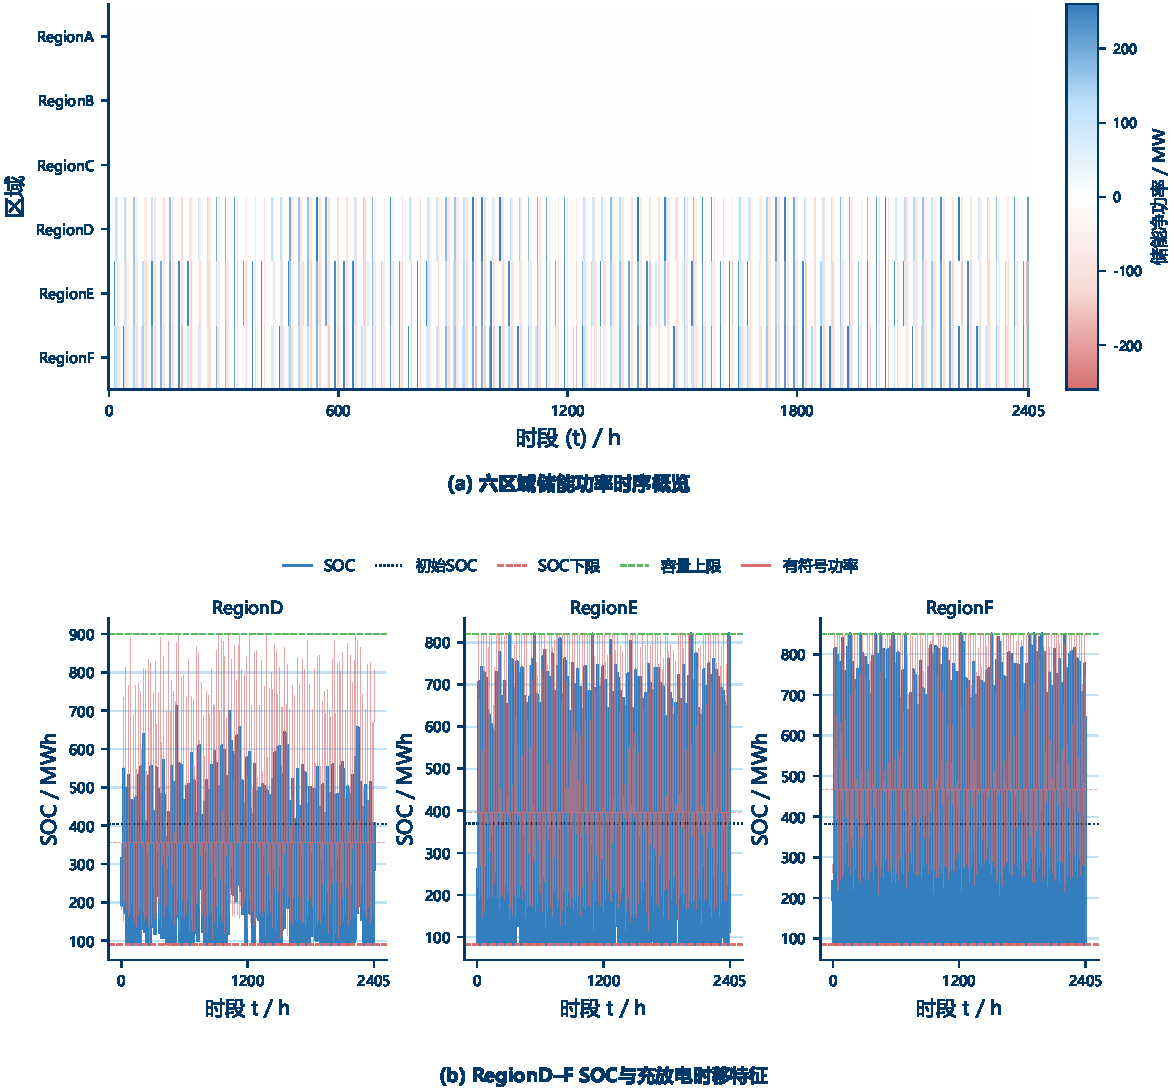
\includegraphics[width=0.92\textwidth]
	{figures/q3_group1_storage_mechanism.pdf}
	\caption{六区域储能功率时序与活跃区域SOC演化特征}
	\label{fig:q3_storage}
\end{figure}

储能由此集中配置于调节需求较强的区域，而非各区域均匀调用。

题目附件状态仅作实际运行对照，不作为满足本文终端SOC条件的同可行域优化基准；无储能方案用于同模型口径消融。
优化后运行成本为
$C=-4.5906\times10^{8}$，
碳排放$E=0$，
六区域峰值净购电之和$P=0$，
平均净购电波动$W=0.0113$ MW。
四项指标均优于附件对照；负成本表示外送收益超过购电支出。

碳排放和峰值净购电均为0，并不表示数据中心没有电力负荷。按照题目给定口径，碳排放仅由电网购电量计算，峰值指标取净购电功率的正部；在当前确定性数据和允许新能源外送的边界下，优化方案利用新能源和储能满足负荷，并将富余新能源外送，因而购电碳排放和正向净购电峰值均降至0。该结论依赖当前新能源、电价、储能和购售电边界，不代表其他参数情景下仍能保持为0。

\begin{figure}[H]
	\centering
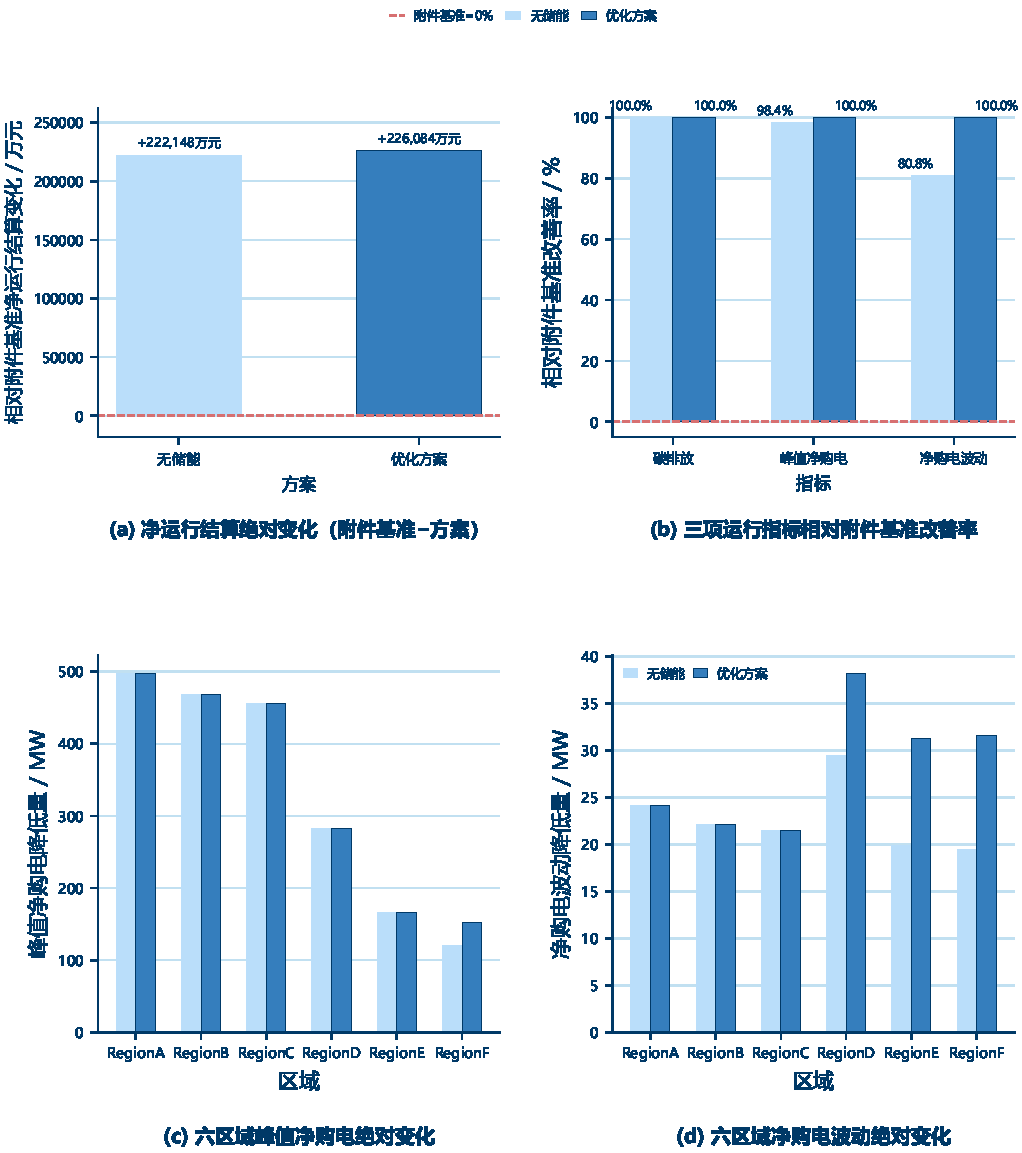
\includegraphics[width=0.86\textwidth]
{figures/q3_group2_optimization_effect.pdf}
\caption{储能协同优化的净运行结算绝对变化、三项指标改善率与区域差异}
	\label{fig:q3_effect}
\end{figure}

图\ref{fig:q3_effect}以万元表示净运行结算绝对变化，以相对改善率表示其余指标，避免成本跨零时的比例歧义。六区域峰值均下降，RegionD--RegionF波动改善更大，与储能活跃区域一致。

令$C^{RE}_{rt}=C^G_{rt}=D_{rt}=0$构造无储能反事实方案。
其运行成本为$-4.1969\times10^{8}$，
碳排放为$8.8506$，
峰值净购电为$31.5979$ MW，
平均净购电波动为$5.3981$ MW。
与其相比，优化方案的净运行成本降低3936.19万元，碳排放、峰值和波动也下降。

独立复核表明，优化方案与无储能方案均满足能源平衡、SOC、容量、互斥、购售电及终端约束。
附件运行对照的新能源平衡和负荷平衡最大残差分别约为
$2.0\times10^{-4}$ MW和$1.504\times10^{-4}$ MW，
处于原始数据精度量级；
但SOC递推最大偏差约为$0.9999$ MWh，
终端SOC缺口约为$193.3$ MWh。
故附件状态可作题设运行对照，但不属于本文约束下的可行优化解。

\begin{figure}[H]
	\centering
	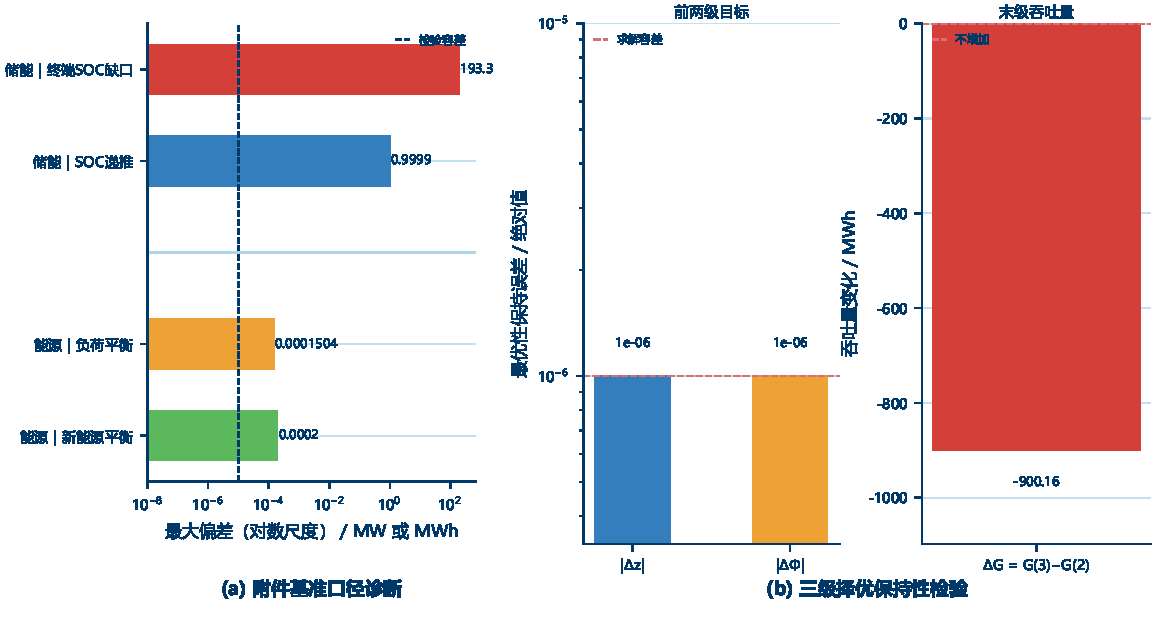
\includegraphics[width=0.91\textwidth]
	{figures/q3_group3_validation_credibility.pdf}
	\caption{附件运行对照口径诊断与多目标三级择优检验}
	\label{fig:q3_validation}
\end{figure}

图\ref{fig:q3_validation}中，第三级使$z$和$\Phi$相对前一级的变化均约$1.0\times10^{-6}$，储能吞吐量减少900.16 MWh，即在保持前两级结果时减少无效循环。

问题三在固定负荷下量化储能的跨时调节作用，并为问题四提供能源侧基准。



\section{问题四的模型建立与求解}

\subsection{模型建立}

问题四联合优化任务区域、开工时刻、新能源、储能及购售电。以问题二可行任务方案为初始方案，沿用问题三能源机理；任务迁移和错峰经PUE映射影响新能源消纳、SOC和电网交换，因而建立算--储--电联合模型。

负荷空间迁移与时间调整可同储能及电力决策联动\cite{ref9}。本文保留任务时限、网络时延、资源容量和能源边界，并设置终端SOC与滚动可恢复约束。

任务侧沿用问题一可行域。由$x_{irs}$和式(\ref{eq:q1_overlap})得到AI IT负荷
$P_{rt}^{AI}=\sum_i\sum_{s\in S_i}p_i\rho_{ist}x_{irs}$，
设施侧负荷为
$F_{rt}=PUE_r(P_{rt}^{AI}+P_{rt}^{NonAI})$。
任务唯一执行，实时任务立即启动，弹性任务满足时窗、时延、GPU、功率及2406边界。

能源侧沿用式(\ref{eq:q3_energy_balance})和式(\ref{eq:q3_soc})及其容量、互斥、购售电与外送约束，并要求$S_{r,2406}\geq S_{r0}$。

为防止滚动求解在前期过度放电，还在每个决策窗口末端加入SOC可恢复条件：
\begin{equation}
	S_{r,\tau+H}
	\geq
	\max\left\{
	S_r^{\min},
	S_{r0}-
	\eta_r^cP_r^{ch,\max}(2406-\tau-H)
	\right\}.
	\label{eq:q4_soc_recovery}
\end{equation}

式(\ref{eq:q4_soc_recovery})保证剩余时域仍有恢复初始SOC的理论能力，并在终点衔接终端约束。

六项评价指标为净运行结算$C$、碳排放$E$、网络时延$L$、等待损失$J$、新能源未利用率$Q$和峰值净购电$P$。前三项口径沿用问题二、三；设弹性任务合法开工边界为$\underline{s}_i,\overline{s}_i$，时延敏感权重为$\omega_i$，则
\begin{equation}
	\begin{aligned}
		J&=
		\frac{
			\displaystyle\sum_{i\in I^{\mathrm{flex}}_+}
			\omega_i
			\frac{s_i-\underline{s}_i}
			{\overline{s}_i-\underline{s}_i}}
		{\displaystyle\sum_{i\in I^{\mathrm{flex}}_+}\omega_i},
		\qquad QoS=1-J,\\
		Q&=
		\frac{\displaystyle\sum_r\sum_tR_{rt}}
		{\displaystyle\sum_r\sum_tP^{RE}_{rt}},
		\qquad U=1-Q,\\
		P&=\sum_rP_r^{\max},
		\qquad
		P_r^{\max}\geq B_{rt}-X_{rt},
		\quad P_r^{\max}\geq0.
	\end{aligned}
	\label{eq:q4_metrics}
\end{equation}

滚动求解前固定全局中心$a_m$和尺度$R_m$，各窗口和情景不再改变；非退化主动指标集合为$\mathcal M_{\mathrm{act}}=\{L,J,Q\}$。
第$\tau$个窗口的标准化偏离和增广极小极大准则为
\begin{equation}
	\begin{aligned}
		d_{m,\tau}
		&=
		\max\left\{
		0,\,
		\frac{\hat f_{m,\tau}-a_m}{R_m}
		\right\},
		\qquad m\in\mathcal M_{\mathrm{act}},\\
		\min\quad Z_\tau
		&=
		z_\tau+\eta\sum_{m\in\mathcal M_{\mathrm{act}}} d_{m,\tau},
		\qquad
		d_{m,\tau}\leq z_\tau\quad(m\in\mathcal M_{\mathrm{act}}),
		\qquad
		\eta=10^{-3}.
	\end{aligned}
	\label{eq:q4_minmax}
\end{equation}

式(\ref{eq:q4_minmax})仅对$\mathcal M_{\mathrm{act}}$计算；$C,E,P$独立复算，用于评价和情景比较。六项指标构成统一评价体系，但并非同等强度的主动优化目标。

全时域联合整数变量规模过大，故采用问题二初始方案驱动的滚动数学启发式：$H=24$ h、$K=48$ h、内部推进4 h，前瞻区只提供未来信息。流程见表\ref{tab:q4_algorithm}。

% ==================== Q4：滚动求解流程 ====================
\begin{table}[H]
	\centering
	\caption{问题四滚动算--储--电联合求解流程}
	\label{tab:q4_algorithm}
	
	\fontsize{10.5pt}{12pt}\selectfont
	\renewcommand{\arraystretch}{0.88}
	
	\begin{tabular}{
			>{\centering\arraybackslash}p{0.08\textwidth}
			>{\raggedright\arraybackslash}p{0.86\textwidth}}
		\toprule
		\textbf{步骤} & \multicolumn{1}{c}{\textbf{主要操作}}\\
		\midrule
		
		1 & 读取问题二任务种子及当前SOC、历史峰值和剩余任务状态。\\
		
		2 & 在$H=24$ h决策区和$K=48$ h前瞻区内重新求解储能与购售电响应。\\
		
	3 & 利用边际线性规划评价弹性任务迁移、错峰对联合目标的潜在影响。\\
		
	4 & 对产生资源冲突的局部调整调用小规模混合整数线性规划模型进行可行性修复。\\
		
	5 & 选取关键任务组成大邻域，同时开放任务与能源变量进行联合大邻域搜索精修。\\
		
		6 & 提交当前$H$小时可行结果，并更新SOC、历史峰值、累计碳排放及剩余任务。\\
		
		\bottomrule
	\end{tabular}
\end{table}


联合大邻域同时开放任务区域、开工时刻和能源变量，仅接受满足全部硬约束且使式(\ref{eq:q4_minmax})目标值改善的方案。所得结果为严格满足硬约束且计算效率较高的可行方案，不宣称获得全局最优解。

顺序基准固定问题二任务方案，再按问题三能源模型优化储能和购售电；两方案采用相同六项指标。

保持任务、网络、容量和储能参数不变，分别改变碳约束、电价机制和新能源波动。设基准碳排放为$E^0$、低碳参考为$E^{LC}$，新能源平滑参数为$\gamma$，三类情景定义为
\begin{equation}
	\begin{aligned}
		E
		&\leq
		E^0-\lambda(E^0-E^{LC}),
		\qquad 0\leq\lambda\leq1,\\
		\pi_{rt}^{fix}
		&=\bar{\pi}_r,
		\qquad
		\sigma_{rt}^{fix}=\bar{\sigma}_r,\\
		P_{rt}^{RE}(\gamma)
		&=
		(1-\gamma)P_{rt}^{RE}
		+\gamma\bar P_{rd}^{RE,+},
		\qquad
		t\in\mathcal H_{rd}^{+}.
	\end{aligned}
	\label{eq:q4_scenarios}
\end{equation}

新能源平滑仅作用于原非零时段并保持每日总量，所有情景沿用固定定标尺度。

最终由任务表和完整SOC轨迹重构第0--2405小时剖面，统一复算六项指标及全部硬约束。

\subsection{求解结果与模型检验}

采用$H=24$ h、$K=48$ h对50000个任务完成101个滚动窗口，仅提交满足全部硬约束的决策区结果，并在全时域统一复算。

旧顺序能源解因报告型指标退化而形成了物理意义较弱的比较基准。为消除该影响，本文固定问题二顺序任务方案和既有联合任务方案，均按相同的能源响应规则重新优化储能与购售电。该步骤仅统一复算两套任务方案的能源轨迹，不等同于重新执行完整联合搜索。结果见表\ref{tab:q4_result}。

% ==================== Q4：联合方案结果 ====================
\begin{table}[H]
	\centering
	\caption{统一能源口径下联合任务方案与顺序任务方案对比}
	\label{tab:q4_result}
	
	\fontsize{10.5pt}{12pt}\selectfont
	\renewcommand{\arraystretch}{0.90}
	
	\begin{tabular}{lrr}
		\toprule
		\multicolumn{1}{c}{\textbf{评价指标}}
		& \multicolumn{1}{c}{\textbf{顺序任务方案}}
	& \multicolumn{1}{c}{\textbf{联合任务方案}}\\
		\midrule
		
		净运行结算/元
		& $-4.532307\times10^8$
		& $-4.538873\times10^8$\\
		
		碳排放/tCO$_2$
		& 30.1233
		& 71.2005\\
		
		平均网络时延/ms
		& 12.9468
		& 9.9618\\
		
		QoS损失
		& 0.083659
		& 0.079281\\
		
		新能源未利用率
		& 29.8615\%
		& 29.8357\%\\
		
		峰值净购电/MW
		& 66.5709
		& 97.1828\\
		
		\bottomrule
	\end{tabular}
\end{table}


表\ref{tab:q4_result}中，联合任务方案的净运行结算降低$6.5665\times10^5$元，时延下降2.9851 ms，QoS损失下降0.004378，新能源未利用率降低0.0258个百分点；碳排放增加41.0772 tCO$_2$，峰值净购电增加30.6119 MW。负结算表示外送收益超过购电支出。结果表明，联合任务调整主要改善服务质量并小幅降低净结算和弃新能源，但未使六项评价指标同时改善。

因此，两类方案不存在脱离决策偏好的统一优劣关系。若调度者优先改善网络时延、等待损失和新能源消纳，并能接受相应的碳排放与峰值净购电增量，则可采用联合任务方案；若碳排放或峰值净购电属于严格控制指标，则应采用相应约束情景下的方案。本文据此将结果解释为不同运行偏好下的可行策略集合，而不指定脱离应用条件的唯一最优方案。

\begin{figure}[H]
	\centering
	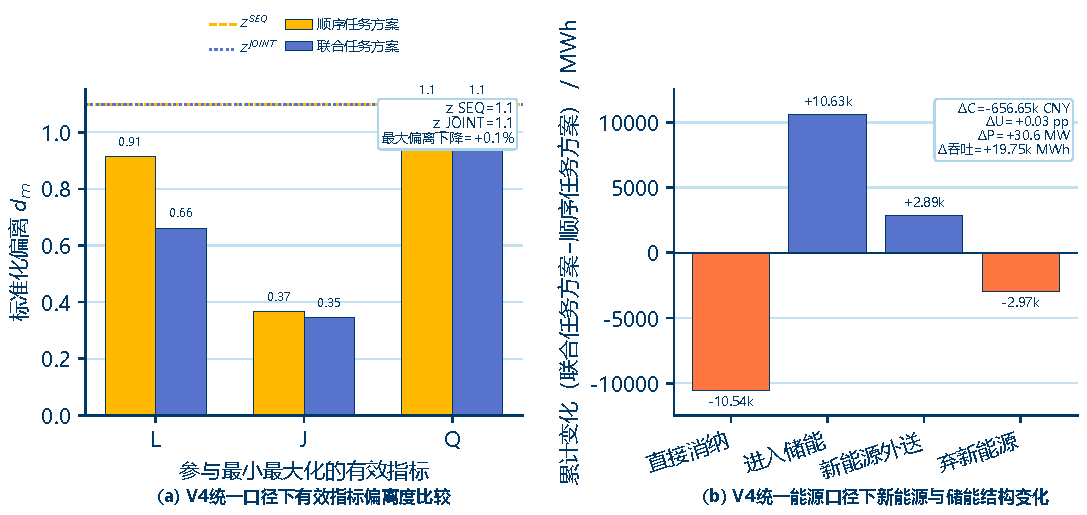
\includegraphics[width=0.88\textwidth]
	{figures/q4_group1_joint_optimization_results.pdf}
	\caption{统一能源口径下两类任务方案的有效指标与新能源--储能结构对比}
	\label{fig:q4_joint_result}
\end{figure}

图\ref{fig:q4_joint_result}中，联合任务方案相较顺序任务方案的新能源直接消纳减少$10.54\times10^3$ MWh，储能充入和外送分别增加$10.63\times10^3$、$2.89\times10^3$ MWh，弃新能源减少$2.97\times10^3$ MWh，储能吞吐量增加$19.75\times10^3$ MWh。图中$L,J,Q$为既有联合搜索实际采用的非退化主动指标；$C,E,P$按统一能源口径独立复算，用于报告任务方案的能源侧代价，不将其追溯表述为联合搜索目标。

按式(\ref{eq:q4_scenarios})构造碳约束、平价电价和新能源平滑情景，相对联合基准的变化见图\ref{fig:q4_scenario}。该图沿用已完成情景组及其同版本联合基准，仅比较组内相对响应；表\ref{tab:q4_result}与图\ref{fig:q4_joint_result}的定点能源复算专用于纠正顺序--联合方案比较，两类结果不交叉拼接绝对量。

\begin{figure}[H]
	\centering
	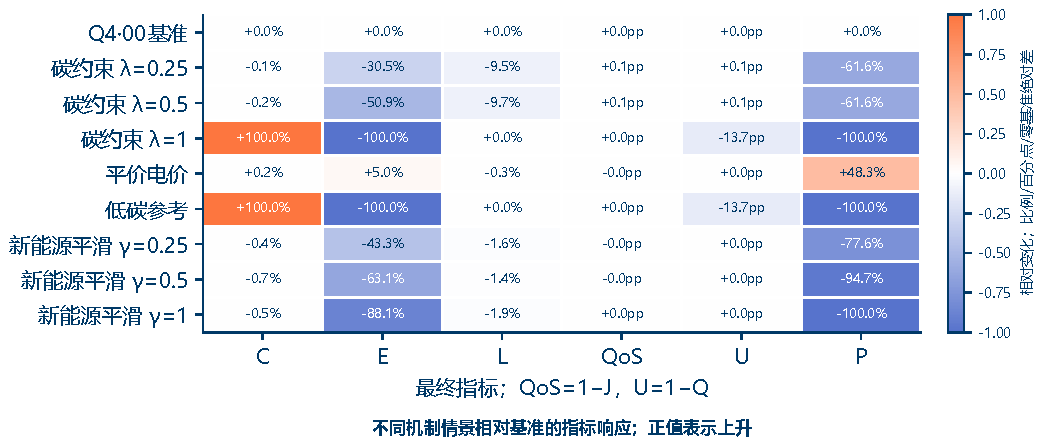
\includegraphics[width=0.86\textwidth]
	{figures/q4_group2_scenario_response.pdf}
	\caption{不同机制情景相对问题四基准的指标响应}
	\label{fig:q4_scenario}
\end{figure}

图\ref{fig:q4_scenario}中，$\lambda$由0.25增至0.50时，碳排放由297.36降至209.97 tCO$_2$，峰值约95.54 MW，时延由9.0144变为8.9945 ms。
当$\lambda=1$时，碳排放和峰值净购电接近0，
但新能源未利用率升至43.5710\%，
即继续压缩购电会牺牲新能源利用，并非各指标同步改善。

平价电价下碳排放449.37 tCO$_2$、峰值升至368.71 MW。新能源平滑情景中，
当$\gamma=0.25,0.50,1.00$时，
碳排放分别约为242.89、158.01和50.85 tCO$_2$，
峰值净购电分别约为55.73、13.18和0 MW，
时延均为9.77--9.81 ms，表明平滑主要改变能源侧状态。

采用全时域独立复算和代表窗口完整混合整数线性规划检验。顺序任务方案与联合任务方案各67项任务、容量、时延、能源、SOC及购售电复核均通过，最大硬约束违反量为
$2.3842\times10^{-7}$，低于$10^{-6}$的检验容差；
六项指标独立复算后与汇总结果的最大差异亦不超过该量级。

\begin{figure}[H]
	\centering
	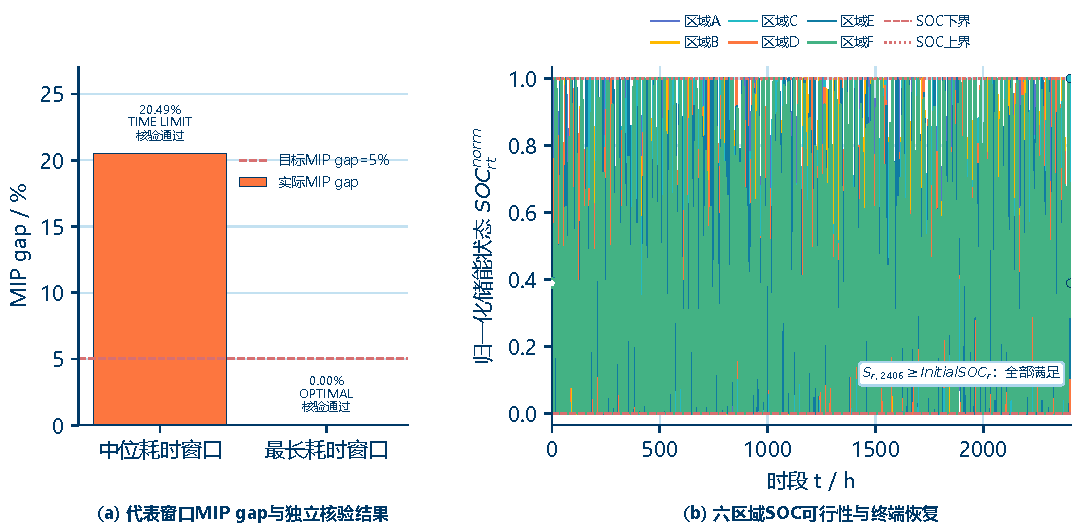
\includegraphics[width=0.88\textwidth]
	{figures/q4_group3_model_validation.pdf}
	\caption{问题四代表窗口完整混合整数线性规划与六区域储能状态的独立检验结果}
	\label{fig:q4_validation}
\end{figure}

图\ref{fig:q4_validation}(a)对1512和2232窗口作完整联合混合整数线性规划对照：前者在600 s内得到相对间隙20.49\%的可行参考解，后者达到最优，二者约束复核均通过。该检验只提供局部可行性与有限解质量参照，不能证明全时域近优或全局最优。

图\ref{fig:q4_validation}(b)给出联合任务方案按统一能源核算口径复算后的SOC轨迹。SOC始终位于上下界内，且$S_{r,2406}\geq S_{r0}$，未通过透支初始储能获取收益。

问题四的联合任务方案在当前数据下改善网络时延、等待损失和新能源未利用率，同时使碳排放与峰值净购电增加，说明联合决策产生的是指标权衡而非六项同步占优。两套任务方案均满足任务、算力、能源和储能硬约束；其结论限于严格满足硬约束且计算效率较高的可行方案，不宣称获得全局最优解，也不将能源定点复算等同于完整联合搜索。




	\section{模型评价与推广}

\subsection{模型优点}

\begin{enumerate}
	\item \textbf{分层预测兼顾异质性与一致性：}
	问题一由三级预测恢复18类交叉需求；验证期、测试期WAPE为0.7241、0.6519，84个滚动窗口均优于24小时同刻基线。
	
	\item \textbf{多目标调度能够刻画实际权衡：}
	问题二采用固定定标，50000个任务经全时域复算满足硬约束；成本降低507.34万元、新能源利用率提高0.223个百分点，同时保留碳排放和时延增加的代价。
	
	\item \textbf{储能模型保持题设负荷口径：}
	问题三固定题设负荷，仅优化能源侧；相较无储能方案，成本降低3936.19万元，碳排放、峰值和波动均下降，SOC及终端约束通过复核。
	
	\item \textbf{联合调度体现算储电协同效应：}
	问题四将顺序任务方案和联合任务方案按统一能源口径复算。联合任务方案使成本降低65.67万元、平均网络时延降低2.9851 ms、新能源未利用率降低0.0258个百分点；碳排放和峰值分别增加41.08 tCO$_2$、30.61 MW，完整呈现了服务质量改善的能源侧代价。两套任务方案各67项独立复核均通过。
\end{enumerate}


\subsection{模型不足}

\begin{enumerate}
	\item \textbf{预测依赖近期需求结构稳定：}
	18类需求恢复依赖历史结构，且相较直接预测的误差变化未达统计显著（$p=0.2163$）；业务突变时需采用动态窗口或时变权重。
	
	\item \textbf{问题二滚动启发式不能保证全局最优：}
	困难窗口与精确模型的最大标准化目标偏差为293.40\%；可按资源紧张度扩大邻域并延长关键窗口求解时间。
	
	\item \textbf{联合模型对极端情景和不确定性考虑有限：}
	问题三、四采用确定性电价、碳强度和新能源序列，未计预测误差与储能衰减；可引入逐级收紧约束及鲁棒或随机优化。
\end{enumerate}


\subsection{推广}

该框架可用于多区域数据中心、算力网络和园区源--荷--储调度，但须按实际任务时窗、网络、容量、PUE、电价、碳强度、新能源、储能和SLA重新标定。若引入任务抢占、电力互济或预测误差，还需扩展状态与不确定性约束并重新检验；可推广的是建模链路，而非本文参数和数值。

	
	% ---------- AI工具使用声明（正文后、参考文献前） ----------
	\section*{AI工具使用声明}
	本参赛队在竞赛过程中使用了DeepSeek，
	主要用于语言润色、代码调试、图表制作与LaTeX排版辅助，
	详细使用情况见附录。
	% ====================== 两个版本二选一，删除不用的版本 ======================
	% 版本1：未使用任何AI工具
%	本参赛队在竞赛过程中未使用任何AI工具。
	
	% 版本2：使用了AI工具，按需修改括号内用途
	% 本参赛队在竞赛过程中使用了AI工具，主要用于【语言润色、代码调试、数据可视化辅助】，详细使用情况见附录。
	% ==========================================================================
	
	\referencescn
	
	\newpage
	% ---------- 附录：软件、复现说明、AI详情与完整源程序 ----------
	\section*{附录}

\subsection*{A. 软件环境与复现说明}

本文采用Python 3.12.13完成计算，使用NumPy、pandas、Matplotlib、Seaborn、OpenPyXL、SciPy和HiGHS完成科学计算、数据处理、绘图和优化求解，使用\texttt{uv}管理运行环境。依赖约束和锁定信息见支撑材料中的\texttt{pyproject.toml}与\texttt{uv.lock}。

复核时先同步运行环境，再按问题一至问题四的顺序执行题目级入口。问题二至问题四的预处理依赖问题一生成的共享处理层，因此不将项目根目录的\texttt{main.py}作为无条件复现入口。运行命令如下：

\begin{lstlisting}[language={},basicstyle=\ttfamily\small]
uv sync
uv run python question\question_01\main.py
uv run python question\question_02\main.py
uv run python question\question_03\main.py
uv run python question\question_04\main.py
\end{lstlisting}

各题入口依次完成数据处理、模型求解、模型检验和结果绘图。支撑材料中同时保留了处理后的模型输入和已生成的结果表。若仅复核论文中的数值，可直接检查结果表及独立检验表；若要从原始附件重新计算，应在保持题目数据不变的前提下重新完成数据处理。

\subsection*{B. 源程序与支撑材料}

支撑材料包含本题全部计算机源程序、运行环境配置、处理后的模型输入、问题一至问题四的关键结果表、模型检验表、论文图形以及文件校验清单。结果表用于追溯正文中的具体数值，图形用于论文展示，独立检验表用于核对任务覆盖、资源容量、能源平衡、储能状态和时间边界等条件。

各问题的支撑结果分别包括：问题一的需求预测、基础算力调度和压力边界检验；问题二的多目标调度、基线对比、资源能源复算和敏感性检验；问题三的储能优化、区域指标、基准复核和约束检验；问题四的算力--储能--电力联合调度、情景比较、代表窗口检验和独立核验。

\subsection*{C. 结果使用边界}

正文中的数值以对应结果表为准，不从图片估读。通过硬约束检验只能说明当前方案在给定数据、参数和边界下具有可行性，不能单独推出全局最优或对所有场景普遍最优。对于采用数学启发式得到的结果，正文如实说明其求解方法、对照检验和剩余局限。

时间边界统一解释为：0--2399小时为主要运行期，2400--2405小时用于处理已到达任务的尾部执行，2406小时为终端结算时点，不作为普通任务运行小时。成本指标若包含售电收益，应按净结算值解释，不等同于实际用电量为负。

\subsection*{D. AI工具使用详情}

本参赛队在竞赛过程中使用了DeepSeek，主要用于语言润色、代码调试、图表制作与LaTeX排版辅助。AI未用于确定核心模型、公式、参数、原始数据和最终结论。

\subsubsection*{D.1 工具与使用日期}

\begin{table}[H]
    \centering
    \small
    \renewcommand{\arraystretch}{1.05}
    \setlength{\tabcolsep}{3pt}
    \begin{tabularx}{0.96\textwidth}{>{\centering\arraybackslash}p{0.18\textwidth}>{\centering\arraybackslash}p{0.20\textwidth}>{\centering\arraybackslash}X>{\centering\arraybackslash}p{0.22\textwidth}}
        \toprule
        AI工具 & 版本/型号 & 开发机构 & 使用日期 \\
        \midrule
        DeepSeek & DeepSeek-v4-flash-0731 & 深度求索（DeepSeek） & 2026年8月7日至8月10日 \\
        \bottomrule
    \end{tabularx}
\end{table}

本文使用的模型版本为DeepSeek‐v4‐flash‐0731。

\subsubsection*{D.2 使用环节与目的}

DeepSeek用于文字润色、程序调试、图表制作、终稿语言压缩、术语统一、正文引用、结果版本一致性检查和LaTeX排版复核。AI未用于生成或篡改原始数据，未改变既有联合任务搜索的目标函数、约束条件和参数设置；新增结果均由本地程序实际运行并独立复算。

\subsubsection*{D.3 关键交互记录}

\noindent\textbf{交互记录1（DeepSeek辅助润色，使用日期：2026年8月7日至10日）}

提示词要求：只检查由参赛队自行完成的论文文字，不增加新的模型、公式、数据或结论，并给出局部修改建议。AI主要指出长句、重复表述、术语不一致和图表衔接问题；参赛队人工筛选、核对并重新表述。

\noindent\textbf{交互记录2（代码调试与图表辅助，使用日期：2026年8月9日）}

提示词要求：仅检查已有程序的语法、索引、数据类型、文件读取和绘图参数，不修改原始数据、目标函数、约束条件、模型结构、参数设置和最终结论。AI提出变量检查、索引调整、数据类型转换和图表标签优化建议；参赛队仅采纳本地运行可复现且不改变模型含义的建议。

\noindent\textbf{交互记录3（DeepSeek终稿复核，使用日期：2026年8月10日）}

提示词要求：严格依据评审清单核对问题四的结果口径，消除顺序基准、联合方案、图表和正文之间的数据混用，并统一学术语体、文内引用和LaTeX排版。AI协助增加固定任务方案的统一能源定向复算与独立核验入口，修改绘图和论文源文件；所有新指标均由参赛队计算机本地运行生成，参赛队负责最终核对和提交。

\subsubsection*{D.4 采纳与人工修改}

AI建议均经参赛队核对后采纳。所有核心方法、公式、参数、结果和结论由参赛队确定；最终程序、数据、图表和结论由参赛队在本地运行并复核。DeepSeek完整记录见支撑材料中的相应使用报告。

程序中的AI辅助说明对应DeepSeek参与的代码检查与修改环节。AI辅助范围限于程序检查、结果复核、图表制作和论文排版，未改写既有联合任务搜索模型。

\subsection*{E. 源程序清单与附件位置}

本题实际使用的全部24个Python源程序不在论文附录中重复排印，统一收录于独立附件\texttt{CCM2601033附件.zip}的\texttt{源程序}目录。附件同时包含\texttt{pyproject.toml}、\texttt{uv.lock}、处理后的模型输入、关键结果表、模型检验表、论文图形及SHA-256校验清单，赛题提供的原始数据未重复收录。

源程序按问题一至问题四的相对目录组织，共24个\texttt{.py}文件；复核时按附录A所列命令依次运行。论文与附件分开提交，附件命名符合“选题+参赛编号+附件”的要求，压缩包大小控制在20 MB以内。


\end{document}
